%%%%%%%%%%%%%%%%%%%%%%%%%%%%%%%%%%%%%%%%%%%%%%%%%%%%%%%%%%%%%%%%%%%%%%%%%%
%% This is a document template for an Otago thesis (Masters or PhD).
%% A skeleton chapter layout is also suggested.
%%
%% Look in the directory example_document for filled-out chapters
%% that show you how to do figures, bibliographies, and tables.
%%
%% Since this was written for Computer Science at Otago University,
%% Harvard (author, date) style citations are used.  Other students
%% should consult their advisors as to what style of citations to use.  
%%
%% Nathan Rountree 9/2/98
%%
%%%%%%%%%%%%%%%%%%%%%%%%%%%%%%%%%%%%%%%%%%%%%%%%%%%%%%%%%%%%%%%%%%%%%%%%%%%

%%
%% In the style of a technical report, in 12pt and one sided.
%% Start chapters on right hand side pages only.
%%
\documentclass[12pt]{report}    
%%\documentclass[12pt,twoside,openright]{report} %% Use this for twosided.

%%
%% Load packages.
%%
\usepackage[bschons]{otagothesis}     %% Use Otago page layout

\usepackage[square,sort,comma,numbers]{natbib} %% Use Natural Sciences bibliography

%%\usepackage{times}              %% Times PostScript font. Don't use
				  %% if thesis contains lots of math.

\usepackage{graphicx}             %% jpg, gif, tiff, and pdf graphics
\usepackage{moreverb}             %% Verbatim Code Listings
\usepackage{array}
\usepackage{subfig}
\usepackage{alltt}
\usepackage{siunitx}
\usepackage{nameref}
\usepackage{csquotes}
\usepackage[hidelinks]{hyperref}
\usepackage{algorithmic}
\usepackage{algorithm}
\usepackage{pgfplots}
\usepackage{setspace}
\newcommand{\ThesisName}{Form segmentation, Recover and Regenerate in English and Bangla using Tesseract OCR Engine}
%%
%% Set title, author and date.
%%
\title{\ThesisName}
\author{Tanvir Hasan\hspace{2cm}Reg No: 12101005\\
		Anup Kumar Kar\hspace{1.1cm}Reg No: 12101033\\
		Sayem Hossain\hspace{1.7cm}Reg No: 12101046}
\date{\today}

%%
%% The library want to know all sorts of personal stuff!
%% Can be left out if you don't use the \frontstuff command
%%


%%
%% Uncomment to just print up a few chapters.
%%
%%\includeonly{literature,conclusion}

%%
%% Go!
%%
\begin{document}
%%
%% Put in titlepage and contents, etc...
%%
\frontstuff


%%
%% Set to one-and-a-half line-spacing
%%
\linespread{1.3} \normalsize

%%
%% Include each chapter as a separate file.
%% These lines assume there are files called intro.tex, literature.tex etc.
%%


\chapter{Introduction}
\label{intro}
Segmentation of Images \cite{Segmentation} is the widely investigated field of image processing, image analysis and important module of early vision problem. It is the process to cluster a form image into some isolated image regions corresponding to individual surface, objects or some natural part of the object. It is the process of separating an image into some disjoint or distinct regions whose characteristic such as intensity; colon texture etc. are similar. No two such regions are similar with respect to these characteristics. in digital image processing, digital image analysis usually involves a 'low-level' and a 'high-level' processing. In low-level analysis, the representation of an image is transformed from a numerical array of pixel intensities to a symbolic set of image primitives: edges and regions. In high-level analysis, object labels (or interpretations) are assigned to these primitives, thereby providing a semantic description of the image.

An image is segmented \cite{Segmentation} for different kind of implementations like object recognition to extract data from it, occlusion boundary estimation within motion or stereo systems, image compression, image editing or image database lookup.

The output of image segmentation is a set of segments that collectively cover the entire image, or a set of contours extracted from the image. Each of the pixels in a region are similar with respect to some characteristic or computed pAn image is segmented for different kind of implementations like object recognition to extract data from it, occlusion boundary estimation within motion or stereo systems, image compression, image editing or image database lookup.

property, such as color, intensity, or texture. Adjacent regions are significantly different with respect to the same characteristic. 
image segmentation is a fundamental part of the 'low level' aspects of computer visions and has many practical applications such as in medical imaging, industrial automation and satellite imagery.Traditional methods for image segmentation have approached the problem either from localization in class space using region information or from localization in position, using edge or boundary information. for monochrome images generally are based on one of two basic properties of gray- level values: discontinuity and similarity. In the first category, the approach is to partition an image based on abrupt changes in gray level. The principal areas of interest within this category are detection of isolated points and detection of lines and edges in an image. The principal approaches in the first category are based on edge detection, and boundary detection. Basically, the idea underlying most edge-detection techniques is the computation of a local derivative operator. The first derivative of the gray-level profile is positive at the leading edge of a transition, negative at the trailing edge, and zero in areas of constant gray level. Hence the magnitude of the first derivative can be used to detect the presence of an edge in an image.
In this paper we are proposing a form segmentation, an image segmentation methodology using threshold techniques that will be applied to a form image and data matching algorithms to detect different objects and clusters.
The goal of segmenting a form image is to extract text data isolating texts of different part of that image by segmenting form into several sections. It becomes easy to extract digital data by processing individual objects into texts if we can first isolate that object scenario and use it for processing.

\section{Objective}
The objective is to decompose the image into parts for further analysis. In simple cases, the environment might be well enough controlled so that the segmentation process reliably extracts only the parts that need to be analyzed further. The segmentation is reliable provided that the person's clothing or room background does not have the same color components as a human face. In complex cases, such as extracting a complete road network from a grayscale aerial image, the segmentation problem can be very difficult and might require application of a great deal of domaina building knowledge.
Another objective of segmentation is to perform a change of representation. The pixels of the image must be organized into higher-level units that are either more meaningful or more efficient for further analysis (or both). A critical issue is whether or not segmentation can be performed for many different domains using general bottom-up methods that do not use any special domain knowledge. This chapter presents segmentation methods that have potential use in many different domains. Both region-based and curve-based units are discussed in the following sections. The prospects of having a single segmentation system work well for all problems appear to be dim. Experience has shown that an implementor of machine vision applications must be able to choose from a toolset of methods and perhaps tailor a solution using knowledge of the application.
\section{Motivation}
In recent years, with the advancement of digital era, we are facing a problem of converting handwritten data into digital data for the purpose of saving them in database or repositories in order to analyse or perform operation on the data or keeping log for the future. We still need to process handwritten documents and forms manually that takes lot of times and resources and increases the possibilities to make mistake when processing that data. That causes serious Inefficiency and pain worth not to do it manually.

Several offices including government and non-government organizations gets a lot of applications and different kind of forms every day that needs to be processed immediately with efficient measure and more accuracy. 
In this paper we have proposed an efficient way to process those analogue data into digital texts through form segmentation, a technique of processing form image into digital text. Experimental results shows it?s accuracy and efficiency to process a form that is lot less time consuming and effective.  

\section{Overview of this book}
In this chapter we have introduced the problem of predicting amino acid interaction network in protein. Rest of the chapters are organized as follows.

In Chapter \ref{background_study}, we will acquire some background knowledge by discussing about protein structure including amino acid, primary, secondary and tertiary structure of protein.

In Chapter \ref{literature_review}, we are going to discuss about some existing researches on protein structure prediction and amino acid interaction network prediction.




\chapter {Background Study}
\label{background_study}
Base of a good research is the understanding of the background terms and definition. To understand the image processing and character reorganisation, one have to clearly understand about image filtering, image transformations and tesseract OCR Engine operation. In this chapter as background knowledge discovery we will discuss about some image processing term and tesseract.

\section{Gray Scale}
In photography and computing, a grayscale or greyscale digital image is an image in which the value of each pixel is a single sample, that is, it carries only intensity information. Images of this sort, also known as black-and-white, are composed exclusively of shades of gray, varying from black at the weakest intensity to white at the strongest. \cite{GrayScale}

\section{Blur}
Blurring is a very powerful operation used in image processing and procedural texture generation. Blurs involve calculating weighted averages of areas of pixels in a source image for each pixel of the final blurred image. Blurring images so they become fuzzy may not seem like a useful operation, but actually is very useful for generating background effects and shadows\cite{GaussianSmoothing}. In our form image blur operation increase border edges.

\subsection{Gaussian smoothing}
The Gaussian smoothing operator is a 2-D convolution operator that is used to `blur' images and remove detail and noise. The idea of Gaussian smoothing is to use this 2-D distribution as a `point-spread' function, and this is achieved by convolution. Since the image is stored as a collection of discrete pixels we need to produce a discrete approximation to the Gaussian function before we can perform the convolution. I Gaussian smoothing technique is widely used effect in graphics software, typically to reduce image noise and reduce detail. \cite{GaussianSmoothing}
\begin{figure}[H]
\centering
\label{fig:Blur} 
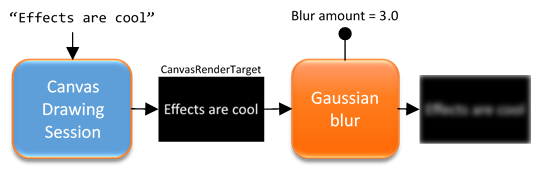
\includegraphics[width=0.8\textwidth]{Blur.png}
\caption {Gaussian smoothing}
\end{figure}

\section{Thresholding}
Thresholding is one of the most basic techniques for what is called Image Segmentation. When the threshold technique is applied on an image, we get segments inside the image and each of segments are represent something.\cite{Thresholding}
\begin{itemize}
\item Thresholding is a simple way of segmentation.
\item We separate out various regions of an image regarding to objects which we want to analyze. The object pixels and the background pixels are the backbone of this separation.
\item To differentiate the pixels we are interested in from the rest, we perform a comparison of each pixel intensity value with respect to a threshold.
\item Once we have separated properly the important pixels, we can set them with a determined value to identify.
\end{itemize}

\begin{figure}[H]
\centering
\label{fig:Thresholding} 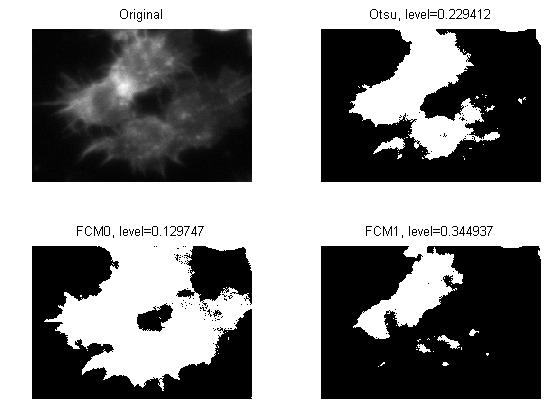
\includegraphics[width=0.8\textwidth]{Thresholding}
\caption {Thresholding}
\end{figure}


\section{Edge Detection}
In digital image processing, edge detection is an important subject matter. Edge detection is a crucial step in object recognition. It is a process of finding sharp discontinuities in an image. The discontinuities are abrupt changes in pixel intensity which characterize boundaries of objects in a scene. In short, the goal of edge detection is to produce a line drawing of the input image. \cite{EdgeDetection}

The Canny operator is also known as the optimal detector, developed by John F. Canny in 1986.  There are multiple steps to implement the Canny operator. First, a Gaussian filters is used to smooth the image to remove noise in an image. Second, compute the gradient magnitude. Third, apply the algorithm to remove the pixels that are not part of an edge. Last step is involved with the use of hysteresis thresholding along edges. Hysteresis is based on two thresholds which are upper and lower. If a pixel gradient is higher than the upper threshold, then the pixel will be marked as an edge and if a pixel gradient is below the lower threshold, then the pixel will be marked as a non-edge\cite{EdgeDetection} \cite{CannyEdgeDetection}.

\begin{figure}[H]
\centering
\subfloat [Original Image of a building]{\label{fig:EdgeOriginal1} 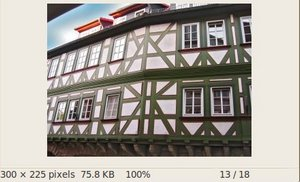
\includegraphics[width=0.6\textwidth]{EdgeOriginal}}
\subfloat [Edge Detected Image]{\label{fig:EdgeDetection1} 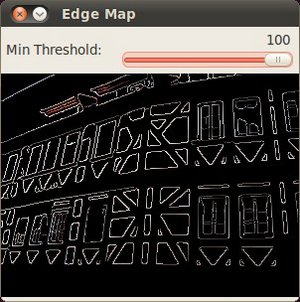
\includegraphics[width=0.5\textwidth]{EdgeDetect}}
\caption {Edge Detection}
\label {fig:EdgeDetection}
\end{figure}

\section{Contour}
Although algorithms like the Canny edge detector can be used to find the edge pixels that separate different segments. The next step is to be able to assemble those edge pixels into contours.
A contour is a list of points that represent, in one way or another, a curve in an image. This representation can be different depending on the circumstance at hand. There are many ways to represent a curve. Contours are represented in OpenCV by sequences in which every entry in the sequence encodes information about the location of the next point on the curve.

\begin{figure}[H]
\centering
\subfloat [Original Image]{\label{fig:ContourOriginal} 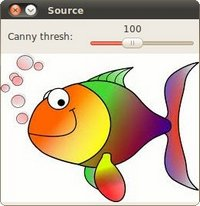
\includegraphics[width=0.4\textwidth]{ContureOriginal}}
\subfloat [Contour Detect]{\label{fig:Contour1} 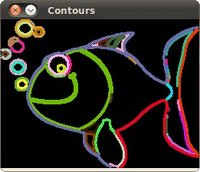
\includegraphics[width=0.4\textwidth]{Conture}}
\caption {Find Contour}
\label {fig:ContourDetection}
\end{figure}

\section{Tesseract OCR engine}
Tesseract is an open source optical character recognition (OCR) engine. HP was originally started it as a project. Later it was modified, improved and taken over by Google and later released as open source in year 2005\cite{TesseractORCEngine} \cite{TesseractORCEngineOfficialWeb}.

Tesseract is considered as one of the most accurate free software OCR engines currently available. A large variety of other OCR software now uses it as a base. It is an excellent quality OCR program, with a large amount of flexibility, a solid codebase, and a large, engaged community of interested people around it.

This thesis investigates the principles of optical character recognition used in the Tesseract OCR engine and techniques to improve its efficiency and runtime. 

Optical character recognition (OCR) method has been used in converting printed text into editable text in various applications over a variety of devices such as Scanners, computers, tablets etc. But now Mobile is taking over the computer in all the domains but OCR still remains one not so conquered field. This paper focuses on improving the Tesseract OCR efficiency for Bangla. 

This thesis presents a preprocessing technique being applied to the Tesseract Engine to improve the recognition of the characters keeping the runtime low.

\section{Why Tesseract}
The first relevant criterion in Tesseract is the fact that is free and open source (FOSS), which is an advantage and a key point in the research development.

Usually, whenever Tesseract is compared to another free OCR tool, it is the best whether in terms of recognition rate or speed. Even, when it is compared with the Finereader commercial tool, Tesseract arrives to rub it and managed to overtake for handwritten writing.

\section{Optical character recognition systems}
An OCR system is a system that takes a text image as input and applies certain treatments through modules making up the system in order to output editable file with the same text.

The architecture of an OCR system varies from one system to another as needed.Optical Character Recognition systems are usually composed of the following phases:

\begin{itemize}
\item Preprocessing phase: prepares the sensor data to the next phase. It is a set of treatments allowing image quality increasing.
\item Segmentation phase: delimits document elements (line, word, character ). By applying good segmentation techniques, we can increase the performance of OCR systems.
\item Feature extraction phase: defines features characterizing the delimited elements of a document. Feature extraction is one of the most important steps in developing a classification system. This step describes the various features characterizing the delimited elements of a document.
\item Classification phase: recognizes and identifies each element. It is performed based on the extracted features.
\item Post-processing phase: it is an optional phase. It may be automatic or manual.
\end{itemize}
Several approaches and techniques have been developed for each module.

\chapter {Literature Review}
\label{literature_review}
The From segmentation process is related to Edge Ditection, Finding contours and contours shapes.And Text ditection related to Tesseract and Tesseact training. Thus in this chapter we will discuss about some state of Image processing technique and Tesseract OCR applications.
\section{Canny Edge Ditection}
The Canny edge detector is an edge detection operator that uses a multi-stage algorithm to detect a wide range of edges in images. It was developed by John F. Canny in 1986. Canny also produced a computational theory of edge detection explaining why the technique works. \cite{EdgeDetection} \cite{CannyEdgeDetection3}
\subsection{Canny Edge Ditection Algorithm}
\begin{enumerate}
\item[\textbf{Step 1}] In order to implement the canny edge detector algorithm, a series of steps must be followed. The first step is to filter out any noise in the original image before trying to locate and detect any edges. And because the Gaussian filter can be computed using a simple mask, it is used exclusively in the Canny algorithm. Once a suitable mask has been calculated, the Gaussian smoothing can be performed using standard convolution methods. A convolution mask is usually much smaller than the actual image. As a result, the mask is slid over the image, manipulating a square of pixels at a time. The larger the width of the Gaussian mask, the lower is the detector's sensitivity to noise. The localization error in the detected edges also increases slightly as the Gaussian width is increased. The Gaussian mask used in my implementation is shown below. 

\begin{figure}[H]
\centering
\label{fig:GaussainMask} 
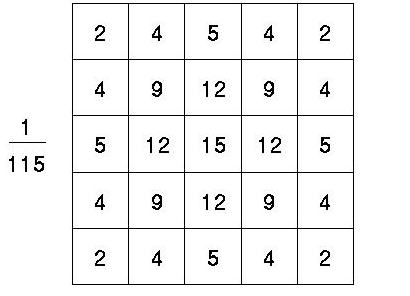
\includegraphics[width=0.5\textwidth]{GaussMask}
\caption {Discrete Approximation to Gaussian function with $\sigma = 1.4$}
\end{figure}


\item[\textbf{Step 2}]After smoothing the image and eliminating the noise, the next step is to find the edge strength by taking the gradient of the image. The Sobel operator performs a 2-D spatial gradient measurement on an image. Then, the approximate absolute gradient magnitude (edge strength) at each point can be found. The Sobel operator uses a pair of 3x3 convolution masks, one estimating the gradient in the x-direction (columns) and the other estimating the gradient in the y-direction (rows). They are shown below:
\begin{figure}[H]
\centering
\label{fig:Mask} 
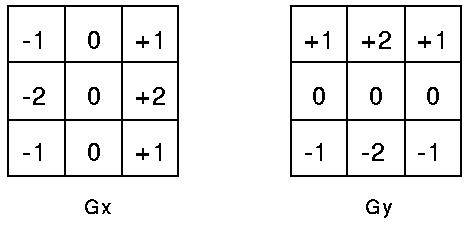
\includegraphics[width=0.6\textwidth]{Mask}
\end{figure}
The magnitude, or EDGE STRENGTH, of the gradient is then approximated using the formula: $|G| = |Gx| + |Gy|$
\item[\textbf{Step 3}]Finding the edge direction is trivial once the gradient in the x and y directions are known. However, you will generate an error whenever sumX is equal to zero. So in the code there has to be a restriction set whenever this takes place. Whenever the gradient in the x direction is equal to zero, the edge direction has to be equal to 90 degrees or 0 degrees, depending on what the value of the gradient in the y-direction is equal to. If GY has a value of zero, the edge direction will equal 0 degrees. Otherwise the edge direction will equal 90 degrees. The formula for finding the edge direction is just: $$\theta = tan^{-1} (Gy / Gx)$$

\item[\textbf{Step 4}]Once the edge direction is known, the next step is to relate the edge direction to a direction that can be traced in an image. So if the pixels of a 5x5 image are aligned as follows: \\
\begin{table}[H]
\centering
\begin{tabular}{|c c c c c|}
\hline
x & x & x & x & x \\
x & x & x & x & x \\
x & x & x & x & x \\
x & x & \textcolor{red}{a} & x & x \\
x & x & x & x & x \\
x & x & x & x & x \\
\hline
\end{tabular}
\caption {Edge Ditection}
\label {tab:Table1}
\end{table} 
Then, it can be seen by looking at pixel "\textcolor{red}{a}", there are only four possible directions when describing the surrounding pixels - 0 degrees (in the horizontal direction), 45 degrees (along the positive diagonal), 90 degrees (in the vertical direction), or 135 degrees (along the negative diagonal). So now the edge orientation has to be resolved into one of these four directions depending on which direction it is closest to (e.g. if the orientation angle is found to be 3 degrees, make it zero degrees). Think of this as taking a semicircle and dividing it into 5 regions.
\begin{figure}[H]
\centering
\label{fig:Canny1} 
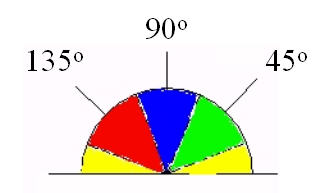
\includegraphics[width=0.6\textwidth]{Canny}
\end{figure}
Therefore, any edge direction falling within the \textcolor{yellow}{yellow range} (0 to 22.5 \& 157.5 to 180 degrees) is set to 0 degrees. Any edge direction falling in the \textcolor{green}{green range} (22.5 to 67.5 degrees) is set to 45 degrees. Any edge direction falling in the \textcolor{blue}{blue range} (67.5 to 112.5 degrees) is set to 90 degrees. And finally, any edge direction falling within the \textcolor{red}{red range} (112.5 to 157.5 degrees) is set to 135 degrees.
\item[\textbf{Step 5}]After the edge directions are known, nonmaximum suppression now has to be applied. Nonmaximum suppression is used to trace along the edge in the edge direction and suppress any pixel value (sets it equal to 0) that is not considered to be an edge. This will give a thin line in the output image.
\item[\textbf{Step 6}]Finally, hysteresis is used as a means of eliminating streaking. Streaking is the breaking up of an edge contour caused by the operator output fluctuating above and below the threshold. If a single threshold, T1 is applied to an image, and an edge has an average strength equal to T1, then due to noise, there will be instances where the edge dips below the threshold. Equally it will also extend above the threshold making an edge look like a dashed line. To avoid this, hysteresis uses 2 thresholds, a high and a low. Any pixel in the image that has a value greater than T1 is presumed to be an edge pixel, and is marked as such immediately. Then, any pixels that are connected to this edge pixel and that have a value greater than T2 are also selected as edge pixels. If you think of following an edge, you need a gradient of T2 to start but you don't stop till you hit a gradient below T1. \cite{CannyEdgeDetection1}\cite{CannyEdgeDetection2}
\section{Contours}
Contours can be explained simply as a curve joining all the continuous points (along the boundary), having same color or intensity. The contours are a useful tool for shape analysis and object detection and recognition. \cite{Contours}
\begin{itemize}
\item For better accuracy, use binary images. So before finding contours, apply threshold or canny edge detection.
\item findContours function modifies the source image. So if you want source image even after finding contours, already store it to some other variables.
\item In OpenCV, finding contours is like finding white object from black background. So remember, object to be found should be white and background should be black.
\end{itemize}
\begin{figure}[H]
\centering
\subfloat [Original Image]{\label{fig:Contour2} 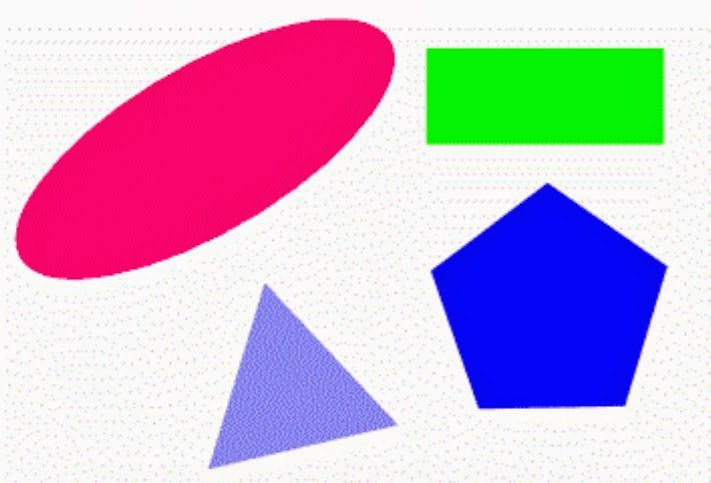
\includegraphics[width=0.5\textwidth]{shape}}
\subfloat [Detected Contours]{\label{fig:DetectContour} 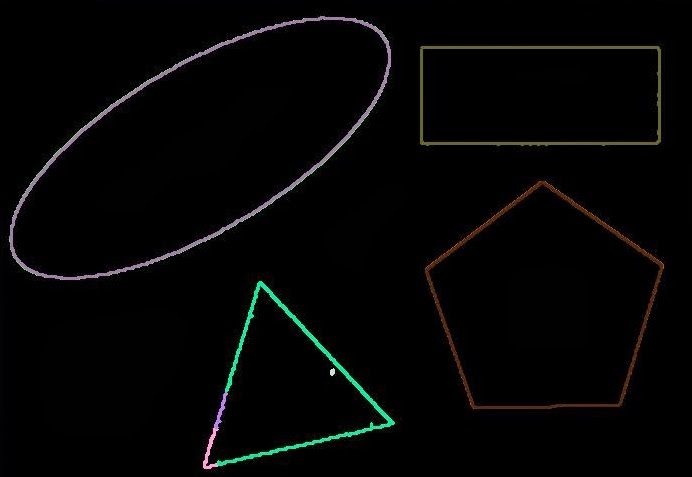
\includegraphics[width=0.5\textwidth]{contours}}
\caption {Find Courours}
\label {fig:Amino_Acid}
\end{figure}
\end{enumerate}
\section{Detecting shapes in images}
Doing image processing and especially blob analysis it is often required to check some objects' shape and depending on it perform further processing of a particular object or not. For example, some applications may require finding only rectangle from all the detected objects, or quadrilaterals, rectangles, etc. \cite{DetectingShape}
\subsection{Detection quadrilaterals}
Detection of quadrilaterals and triangles has pretty much the same idea - we are checking mean distance between provided shape's edge pixels and the edge of estimated quadrilateral/triangle. The only difference here is the way how to estimate parameters of the shape we want to recognize and how to check distance to the estimated shape.

Let's start with quadrilaterals first. For a given shape we can make an assumption that it is a quadrilateral, find its four corners and then using similar method as we've used for circles we can check if our assumption is correct or not - check how good the shape fits into the quadrilateral with assumed parameters.
\begin{figure}[H]
\centering
\label{fig:shape} 
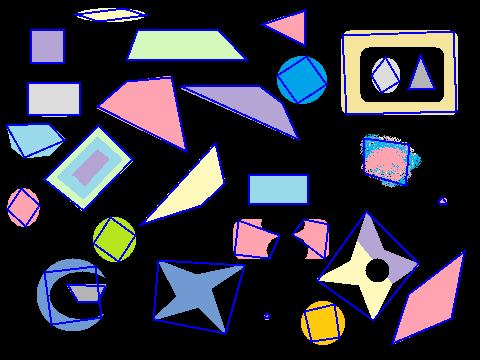
\includegraphics[width=0.6\textwidth]{shapefourcorner}
\caption {Detection of quadrilaterals}
\end{figure}
As we can see on the image above, we may have different objects and quadrilateral finder provides different results for them. For shapes which really look like quadrilateral, the quadrilateral finder is able to find their corners more or less correctly (problem may occur in the case if object has rounded corners). But for other types of objects (circles, starts, etc.), quadrilateral finder does not provide any good result. And this is correct, since this routine supposes the given shape is really quadrilateral.

Now, when we made the assumption that a subjected object is quadrilateral and we got its corner, we just need to see how good is the fit of the object into the quadrilateral with those found corner - we need to make sure there are no edge points of the given shape which are too far away from the edge of the assumed quadrilateral.
\subsection{Detection Rectangles, squares, equilateral}
Once we made a check for quadrilateral shape and got its 4 corners, we may do some further checks to detect sub-type of the quadrilateral: trapezoid, parallelogram, rectangle, rhombus or square. These checks are based on checking angles between opposite/adjacent sides and their length. First we check two opposite sides - if they are parallel, then we get at least trapezoid. Then we check two other sides - if they are parallel two, then we have parallelogram. If two adjacent sides are perpendicular, then we got rectangle. The last check is to compare length of two adjacent sides - if they are equal, then parallelogram becomes rhombus and rectangle becomes square. And of course we need to add small possible error, so if angle between lines equals to 2 degrees, they are still treated as parallel. \cite{DetectingShape}
\section{Tesseract OCR Engine}
\subsection{What is Tesseract?}
An Overview of the Tesseract OCR Engine describes Tesseract as: "Tesseract is an open source
optical character recognition(OCR) engine. HP originally was originally started it as a project. Later it was modified, improved and taken over by Google and later released as open source
in year 2005. It is now available at" (Smith, 2007) . It is very portable as compared to others
and supports various platforms. Its focus is more towards providing less rejection and improved
accuracy. Currently only command base version is available but there are many projects with UI
built on top of it which could be forked. As of now Tesseract version 3.02 is released and
available for use. Now Tesseract is developed and maintained by Google. It provides support for
around 139 languages.
\subsection{Architecture}
Tesseract OCR is an elegant engine with various layers. It works in step by step manner as
shown in the block diagram in fig:3.4 The first step in the cycle is to sense the color intensities of the image, named as adaptive thresholding, and converts the image into binary images.
Second step is to do the connected component analysis of the image, which does the task of
extracting character outlines. This step is the main process of this cycle as it does the OCR of
image with white text and blacks rest of the image.
Tesseract was probably the first to use these cycles to process the input image. After this the
outlines extracted from image are converted into Blobs(Binary Long Objects). It is then organized as lines and regions and further analysis is for some fixed area. After extraction
the extracted components are chopped into words and delimited with spaces. Recognition in text
then starts which is a two pass process. As shown in fig 1, the first part is when attempt to
recognize each word is made. Each satisfactory word is accepted and second pass is started to
gather remaining words. This brings in the role of adaptive classifier. The adaptive classifier then will classify text in more accurate manner. The adaptive classifier needs to be trained beforehand
to work accurately. When the classifier receives some data, it has to resolve the issues and assign
the proper place of the text.

\begin{figure}[H]
\centering
\label{fig:flow} 
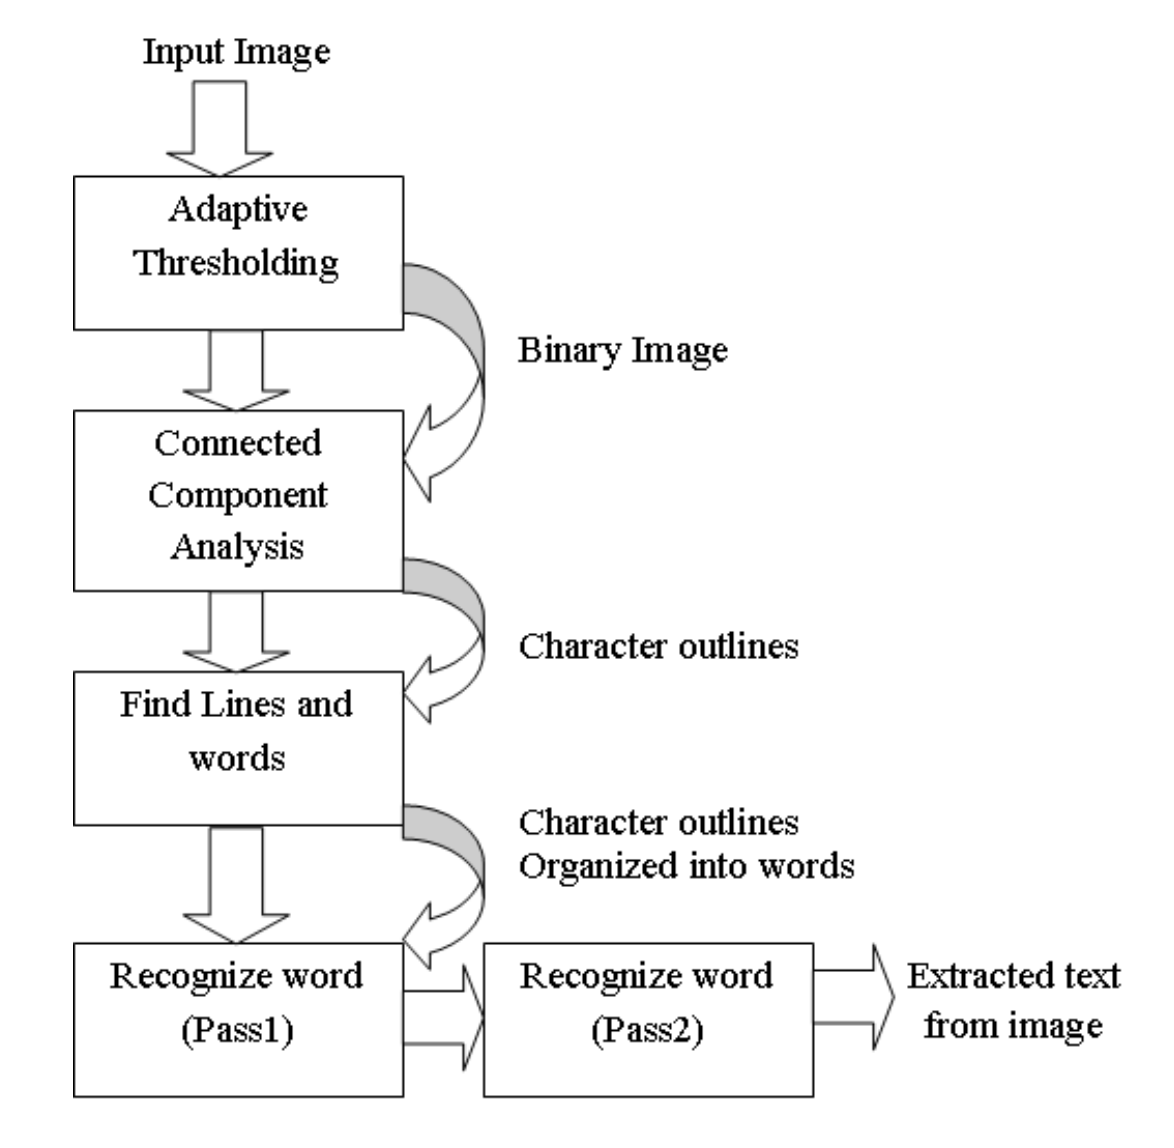
\includegraphics[width=0.8\textwidth]{tesseractFlow}
\caption {Tesseract Flow}
\end{figure}

\subsection{Working of Tesseract}
Tesseract works pretty much as a scanner. Its interface is pretty simple as it takes input o the command lines with very basic commands. We need to input any image with text in it.

The basic Tesseract command takes only two arguments: First is input image that contains text and second argument is output text file which is usually text file.

Tesseract by default picks the extension of output file as .txt. There no need to specify the explicitly the output file extension.Tesseract supports various languages. Each language comes with a trained language data file.

The language file must be kept in a location Tesseract knows. When using in the project it is advised to keep it within the project folder. This folder is Tesseract home folder in your machine. In this research, we are aiming to extract English and Bangla characters from the images so we have to keep both Bangla and English data files.
 
\subsection{How does Tesseract work?}
\textbf{The following is a brief overview of how Tesseract works:}
\begin{enumerate}
\item Outlines are analysed and stored 
\item Outlines are gathered together as Blobs
\item Blobs are organized into text lines
\item Text lines are broken into words 
\item First pass of recognition process attempts to recognize each word in turn 
\item Satisfactory words passed to adaptive trainer 
\item Lessons learned by adaptive trainer employed in a second pass, which attempts
recognize the words that were not recognized satisfactorily in the first pass 
\item Fuzzy spaces resolved and text checked for small caps
\item Digital texts are outputted 
\end{enumerate}
\textbf{During these processes, Tesseract uses:}
\begin{enumerate}
\item algorithms for detecting text lines from a skewed page 
\item algorithms for detecting proportional and non proportional words (a proportional
word is a word where all the letters are the same width) 
\item algorithms for chopping joined characters and for associating broken characters 
\item linguistic analysis to identify the most likely word formed by a cluster of
characters 
\item two character classifiers: a static classifier, and an adaptive classifier which
employs training data, and which is better at distinguishing between upper and
lower case letters 
\end{enumerate}

\subsection{Limitations of Tesseract}
\textbf{Tesseract is an OCR engine, not a complete OCR program.}
Tesseract is an OCR engine rather than a fully featured program similar to commercial
OCR software such as Nuance’s Omnipage. It was originally intended to serve as a
component part of other programs or systems. Although Tesseract works from the 
command line, to be usable by the average user the engine must be integrated into
other programs or interfaces, such as FreeOCR.net, WeOCR or OCRpous. Without
integration into programs such as these, Tesseract has no page layout analysis, no
output formatting and no graphical user interface (GUI).
\section{Training Tesseract}
The setup for English \& Bangla OCR within Tesseract is another important task. The way train the engine and input the dataset matters a lot.
Training Tesseract for English \& Bangla includes four steps mainly and they are as follows:
\subsection{Generating training images}
Tesseract official website explains these steps very well "The first step is to determine the full
character set to be used, and prepare a text or word processor file containing a set of examples"
[31]. The two important points to remember for a training file are: Firstly make sure the file
contains all the characters that we are expecting. Secondly there should be at least 5 samples.
There should be more samples of the more frequent characters - at least 20 [31]. Keeping all this
in mind let's explore how do we create box files.
\subsection{Make box files}
Box file is defined as a sample to match with the characters. We need a 'box' file for each
training image. Tesseract official website defines the box file as "The box file is a text file that
lists the characters in the training image, in order, one per line, with the coordinates of the
bounding box around the image" [31]. Tesseract is not so intuitive about the sample data.
Inconsistencies may lead to wrong interpretation of data.
\subsection{Run Tesseract}
In this step we run the Tesseract engines with the new training files. The purpose is to create the
trained dataset which works as a rule engine. Also it creates log files.
\subsection{Compute character set} 
Guidelines from Tesseract website state that "Tesseract needs to know the set of possible characters it can output. To generate the unichar set data file, use the unicharset\textunderscore extractor program on the box files generated above":extractor language. fontname. box 
One more requirement in this is, Tesseract needs to have access to character properties i.e.
isalpha, isdigit, isupper, islower, ispunctuation [31].
The system described in [30],[31] have classified Hindi OCR and its setup, training very nicely.
The only limitation is that the system is for desktop. We have to build the similar system for
mobile devices.
\section{OpenCV}
OpenCV[1] (Open Source Computer Vision) is a library of programming functions and algorithms
[36]. Their main focus is to provide API mainly aimed at real-time computer vision. It was
originally developed by Intel. OpenCV library is free for use for development (under the open
source BSD license) [36]. The best feature is that the library is cross-platform . 

\chapter{Proposed Method}
\label{chap:algorithm}
In this thesis we have implemented a well define digital process to recognize hand writings from a registration form or any kind of forms which are mostly documentation of government or private institutions. Image recognition is a process, which usually consist of taking a picture, process the image then present the results.The whole work can be divided into two parts:
\section{Data Extraction}
We work on a defined format of from. In this process the from every field should be separate by box region.
\begin{figure}[h!]
\centering
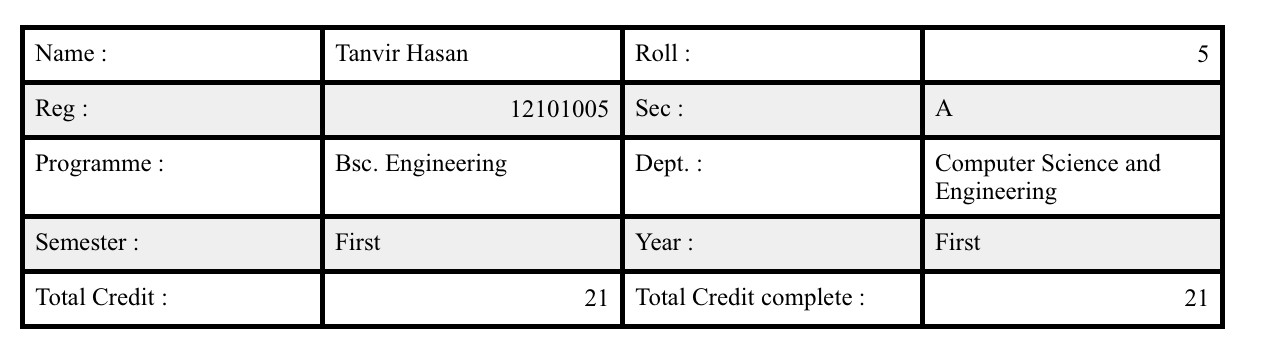
\includegraphics[width=1\textwidth]{from}
\caption {Form template}
\label {fig:FormTemplate}
\end{figure}
\subsection{Convert RGB to Gray Image}
First we have to take input form as picture.Then convert RGB image to gray image.
\begin{figure}[h!]
\centering
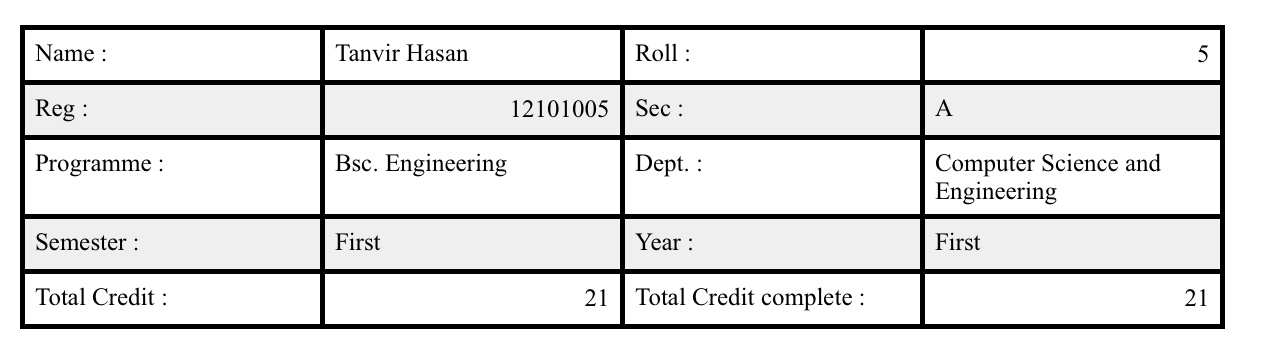
\includegraphics[width=1\textwidth]{GrayImage}
\caption {RGB to Gray}
\label {fig:GRAY}
\end{figure}
\subsection{Image Smoothing}
Smoothing, also called blurring, is a simple and frequently used image processing operation.  There  are  many  reasons  for  smoothing,  but  it  is  usually  done  to  reduce  noise  or  camera artefacts. Smoothing is also important when we wish to reduce the resolution of an image in a principled way\cite{OpenCVBook}.
For our thesis work we used Gaussian blur and this is probably the most useful though not the fastest.
\begin{figure}[h!]
\centering
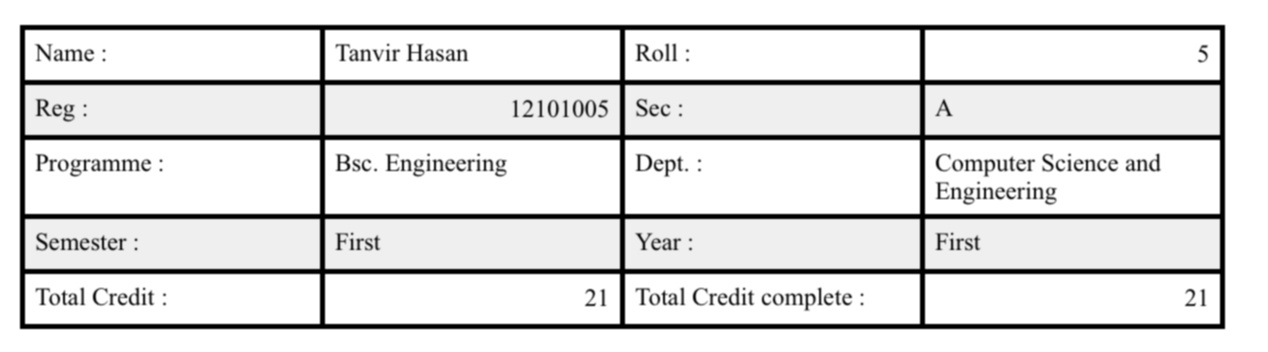
\includegraphics[width=1\textwidth]{GaussianBlur}
\caption {Image after applying gaussian blur in sample form}
\label {fig:GaussianBlur}
\end{figure}
\subsection{Thresholding}
Next we work on image thresholds. Frequently we have done many layers of processing steps and want either to make a final decision about the pixels in an image or to categorically reject those pixels below or above some value while keeping the others. The OpenCV function Threshold() accomplishes these tasks. The basic idea is that an array is given, along with a threshold, and then set a value for every element of the array depending on whether it is below or above the threshold\cite{OpenCVBook}.
\begin{figure}[h!]
\centering
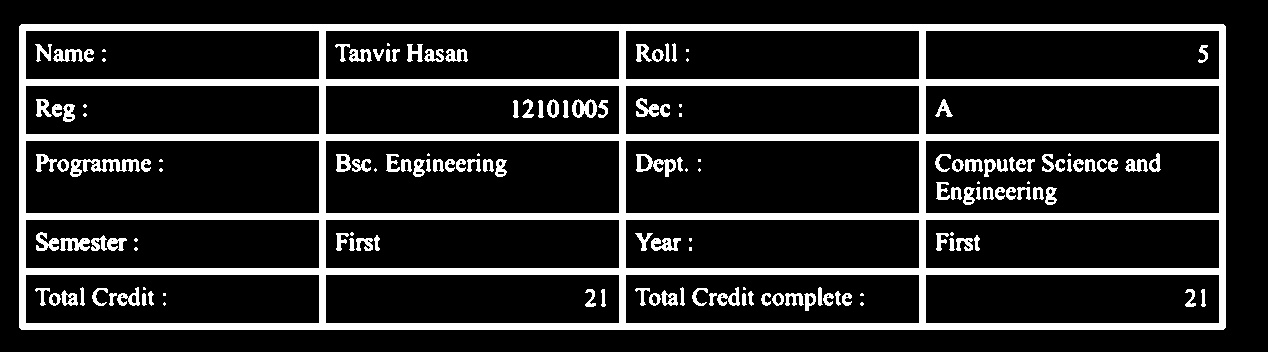
\includegraphics[width=1\textwidth]{Threshold}
\caption {Thresholded image after appling thresholding in sample form}
\label {fig:threshold}
\end{figure}
\subsection{Edge Detection}
We work on the process of edge recognition of an image. For this we used canny edge detector. The method just described in chapter \ref{EdgeDitectionR} for finding edges. The Canny()  function expects an input image, which must be gray scale, and an output image, which must also be gray scale (but which will actually be a Boolean image).\cite{OpenCVBook}
\begin{figure}[h!]
\centering
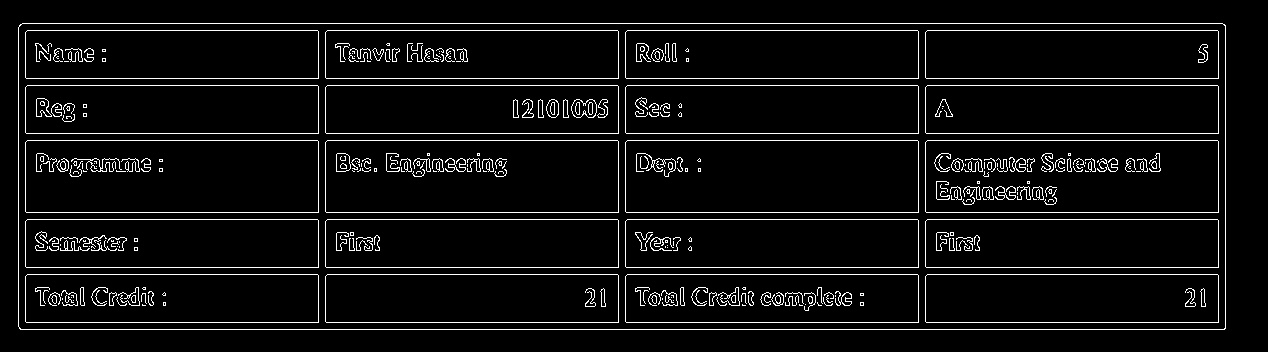
\includegraphics[width=1\textwidth]{Canny2}
\caption {Canny Edge detected image after applying canny edge detection in sample form}
\label {fig:Canny}
\end{figure}
\subsection{Finding Contour}
After edge detection we find out the contours on these defined edges. For this we using opencv function findContours().
\subsection{Select only rectangle shape region}
There can be many regular and irregular shape of contours. But we need only rectangular shape contour. After find contours we filter out irregular shape and keep only the rectangular shape contours. In the \ref{Shape} section we describe how to find rectangle shape.
\subsection{Store only unique region}
For thicker edge one region can be occur multiple time. For this reason we need to filter out only unique region. To doing this we map these region with their left most point coordinate x,y. In every selected left most x,y coordinate we must find unique rectangle region. This is the most efficient way. Otherwise mapping whole region point will be costly.
\subsection{Mapping From Field and Value}
For mapping from different type of field with value, we first store every unique region left-upper most x,y 2D point. Then we sort these 2D point respectively y coordinate then x coordinate. Then we take pair of region form sorted region. The first element of pair will be from filed and second field will be value.
\section{Data Reorganization}
After extracting data from an analogue image, we work on recognize our extracted data by using Tesseract open source engine.  Tesseract converts  the  input  image  into  binary  format  using thresholding. Outlines of  components are  stored  on  connected component   analysis.   Nesting   of   outlines   is   done   which gathers  the  outlines  together  to  form  a  Blob. Text  lines  are analyzed  for  fixed  pitch  and  proportional  text.  Then  the  lines are  broken  into  words  by  analysis  according  to  the  character spacing.   Fixed pitch   is chopped   in   character   cells   and proportional  text  is  broken  into  words  by  definite  spaces  and fuzzy spaces\cite{OCR}.

Tesseract recognises a word in two passes, one is tries  to recognize  the  words in  the  first  pass. If  the  match  is found, then  the  found word  is  passed on to the qdaptive  classifier, which recognizes the text more accurately. During the second pass, the  words  which  were  not at  all recognized or  were  not well recognized in the first pass are recognized again through a run  over through the  page.  Finally  Tesseract  resolves  fuzzy spaces.  To locate  small  and  capital  text, Tesseract  checks alternative hypothesis for x-height OCR engine\cite{OCR} \cite{TesseractORCEngineOfficialWeb}.
\section{Tesseract Training}
For better accuracy we need to train tesseract OCR engine with different type of data.\\
The training procedure of tesseract is well describe in official website of tesseract\cite{TrainingTesseract}\cite{OCR}. 
In short, the training step go through these following steps:
\begin{enumerate}
\item Generate Training Images
\item Make Box Files
\item Edit Box Files
\item Run Tesseract for Training
\item Compute the Character Set
\item set unicharset properties
\item font properties
\item Clustering
\item Putting it all together and make tessdata file.
\end{enumerate}

\chapter {Performance Analysis}
\label{chap:result}
As we have described the proposed method in the chapter \ref{chap:algorithm}. In this chapter we will discuss about result and performance.
\section{Environments of Experiments}
Text examples in public datasets usually occur within high-quality (high-resolution, well-focused) imagery. In our setting, text often occurs at lower-resolution and with significant blur. Our focus is to achieve text spotting in a real-time system moving through an environment. We first examine how much the information is attached with an analogue image than we detect the text and extract the data. Next, we train the data. Finally, we evaluate the accuracy.
We tested with many different categories of the images such as images are taken with mobile camera, scanning images, DSLR camera and handy cam. The accuracy of the output varied greatly. Accuracy varies mainly for image quality. An image is taken with DSLR camera produces most accurate results for it's picture quality. Image of DSLR camera is less noise free. So, it’s easy to extract data and OCR can detect the data perfectly. For handy cam images accuracy is slightly get down. Because picture quality is not good as DSLR camera and there is more noise.
If we use scanned images, it it produces more accurate result than handy cam. Because there is less noise than handy cam images. But for mobile camera images the accuracy level is not so good as regarding the other three image categories. For mobile camera there is more noise and image quality is not good.   

\section{Performance for English form}
We test our proposed algorithm in different types of sample form. The result depends on the tesseract training data. For english we train "Arial","Courier","Calibri","Times New Roman" fonts. Here we show our some output result and analysis of our training data.
\subsection{Sample form 1}

\begin{figure}[H]
\centering
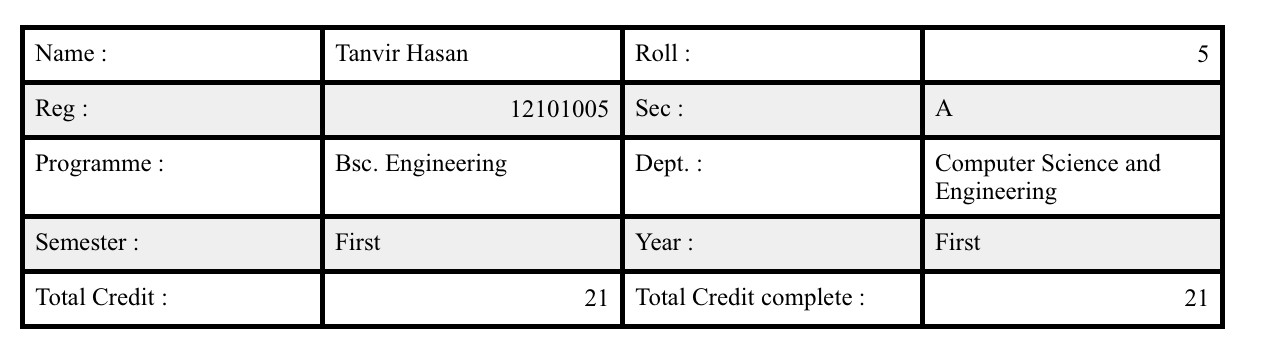
\includegraphics[width=1\textwidth]{form1}
\caption {Sample English form 1}
\label {fig:form1}
\end{figure}

\begin{table}[H]
\centering
\begin{tabular}{|p{2cm}|p{2cm}|p{2cm}|}
\hline
character & Input Frequency & Output Frequency \\
\hline
0 & 3  & 3 \\
\hline
1 & 5  & 7 \\
\hline
2 & 3  & 3 \\
\hline
5 & 2  & 2 \\
\hline
8 & 0  & 4 \\
\hline
: & 10 & 10 \\
\hline
A & 1  & 1 \\
\hline
B & 1  & 1 \\
\hline
C & 3  & 3 \\
\hline
D & 1  & 1 \\
\hline
E & 2  & 1 \\
\hline
F & 2  & 2 \\
\hline
G & 1  & 2 \\
\hline
H & 0  & 2 \\
\hline
I & 1  & 1 \\
\hline
N & 1  & 1 \\
\hline
P & 2  & 2 \\
\hline
R & 3  & 3 \\
\hline
S & 3  & 3 \\
\hline
T & 2  & 2 \\
\hline
Y & 9  & 9 \\
\hline
a & 5  & 5 \\
\hline
c & 3  & 3 \\
\hline
d & 18 & 18 \\
\hline
e & 10 & 8 \\
\hline
i & 2  & 1 \\
\hline
l & 6  & 6 \\
\hline
m & 8  & 7 \\
\hline
o & 6  & 6 \\
\hline
p & 3  & 3 \\
\hline
r & 11 & 11 \\
\hline
s & 5  & 5 \\
\hline
t & 10 & 10 \\
\hline
u & 1  & 1 \\
\hline
v & 1  & 1 \\
\hline
\end{tabular}
\caption { Comparison between Input and Output frequency of Sample Input 1}
\label {tab:Table1}
\end{table}

\begin{figure}[H]
\centering
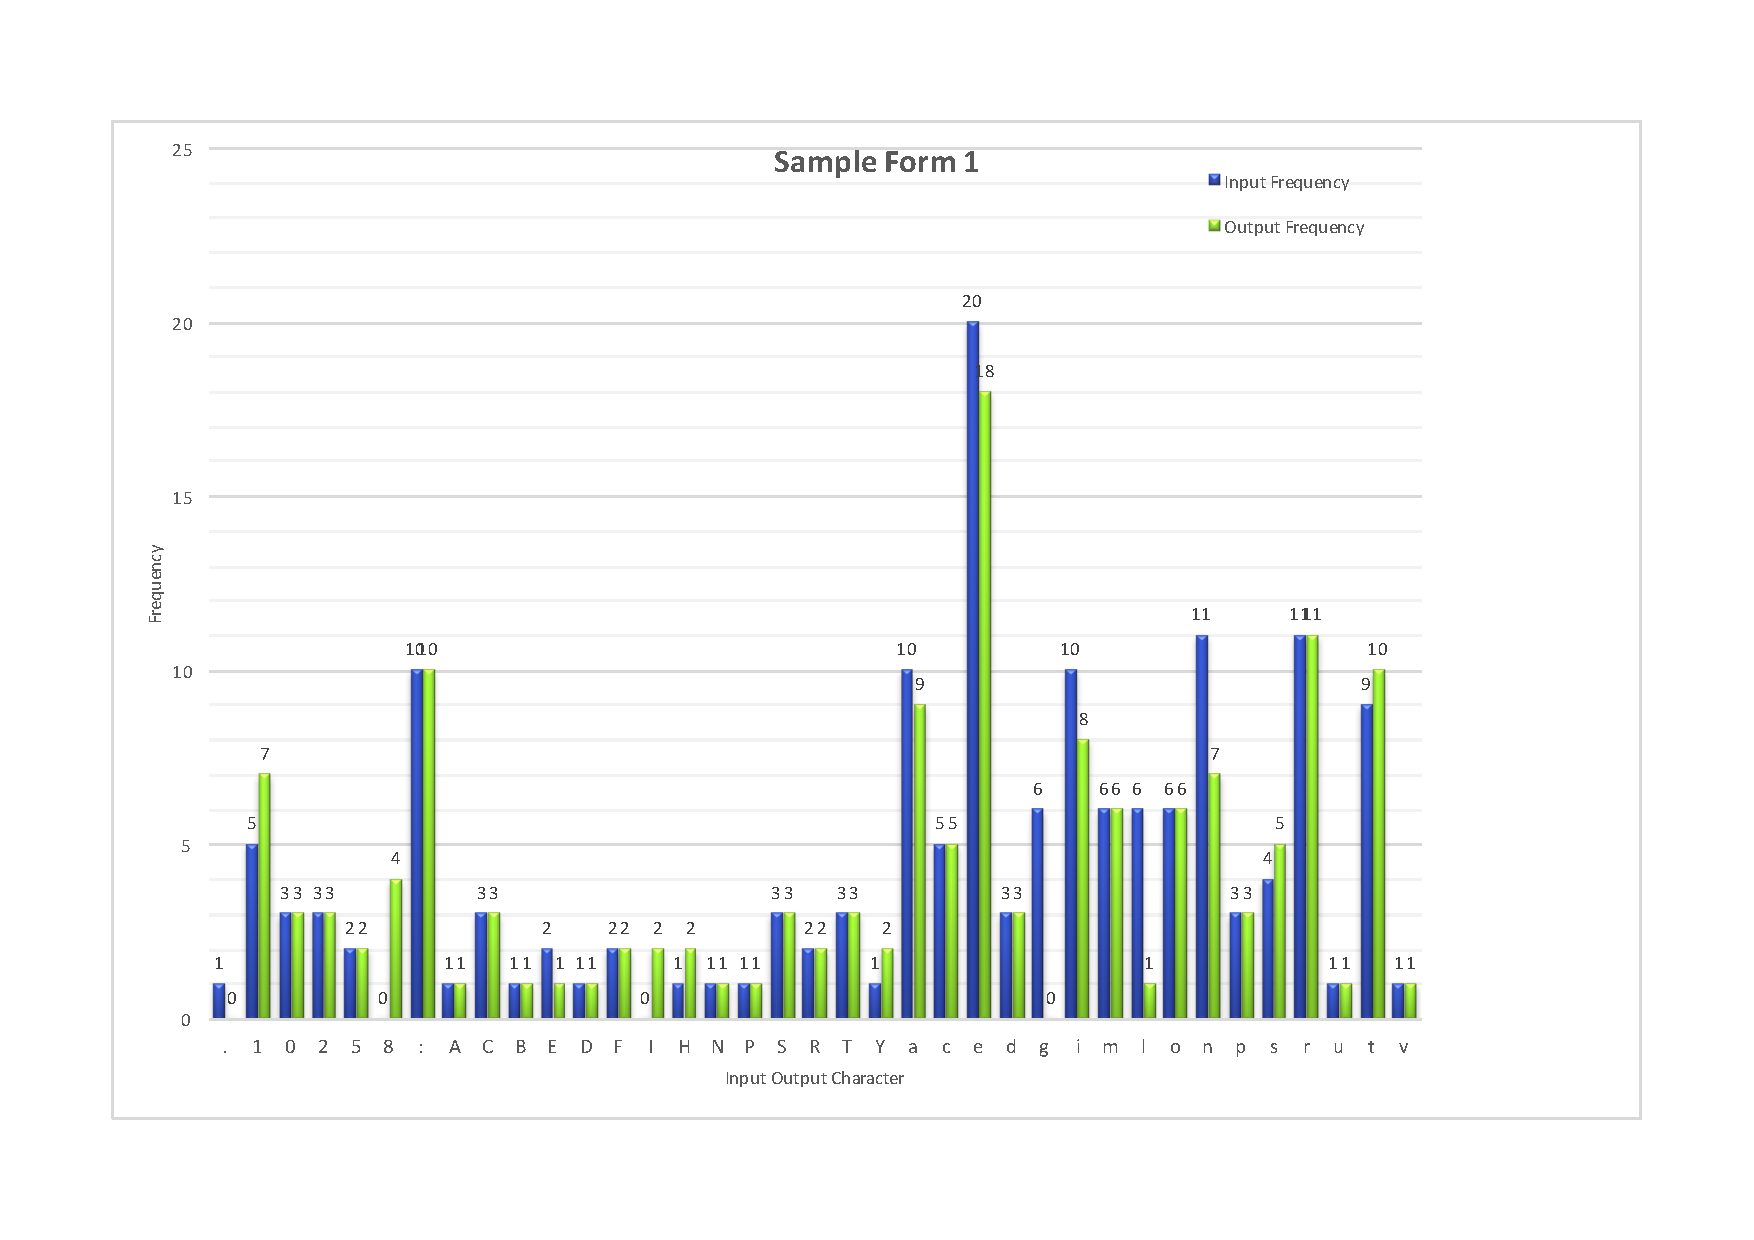
\includegraphics[width=1\textwidth]{form1.pdf}
\caption {Bar chart Input Output Frequency of Sample form 1}
\label {fig:bar1}
\end{figure}

\subsection{Sample form 2}

\begin{figure}[H]
\centering
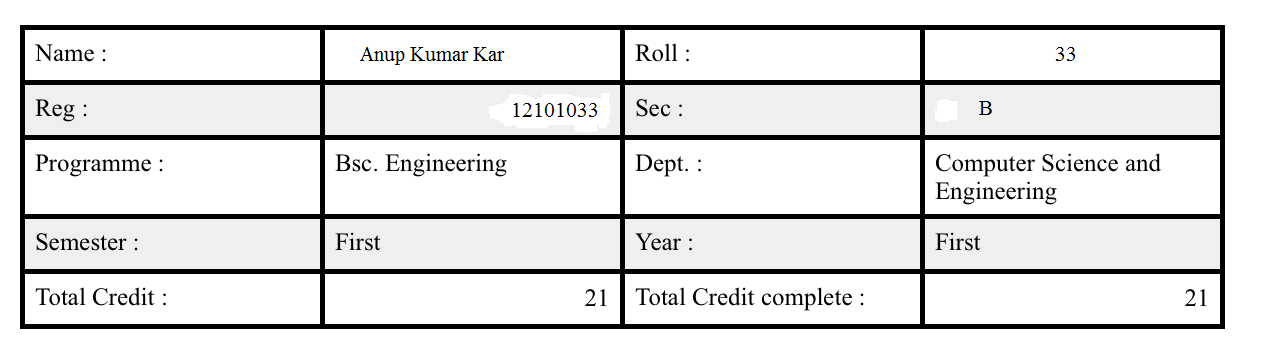
\includegraphics[width=1\textwidth]{form2}
\caption {Sample English form 2}
\label {fig:form2}
\end{figure}

\begin{table}[H]
\centering
\begin{tabular}{|p{2cm}|p{2cm}|p{2cm}|}
\hline
character & Input Frequency & Output Frequency \\
\hline
0 & 2 & 1\\
\hline
1 & 5 & 7\\
\hline
2 & 3 & 3\\
\hline
3 & 4 & 4\\
\hline
8 & 0 & 4\\
\hline
: & 10 & 10\\
\hline
A & 1 & 1\\
\hline
B & 2 & 2\\
\hline
C & 3 & 3\\
\hline
D & 1 & 1\\
\hline
E & 2 & 1\\
\hline
F & 2 & 2\\
\hline
H & 0 & 1\\
\hline
I & 0 & 4\\
\hline
K & 2 & 2\\
\hline
N & 1 & 1\\
\hline
O & 0 & 1\\
\hline
P & 1 & 1\\
\hline
R & 2 & 2\\
\hline
S & 1 & 3\\
\hline
T & 2 & 2\\
\hline
Y & 1 & 2\\
\hline
a & 7 & 8\\
\hline
c & 4 & 5\\
\hline
d & 3 & 3\\
\hline
e & 18 & 18\\
\hline
i & 10 & 7\\
\hline
l & 5 & 1\\
\hline
m & 7 & 7\\
\hline
n & 7 & 6\\
\hline
o & 5 & 6\\
\hline
p & 12 & 4\\
\hline
r & 1 & 10\\
\hline
s & 3 & 4\\
\hline
t & 9 & 10\\
\hline
u & 3 & 3\\
\hline
\end{tabular}
\caption {Comparison between Input and Output frequency of Sample Input 2}
\label {tab:Table2}
\end{table}

\begin{figure}[H]
\centering
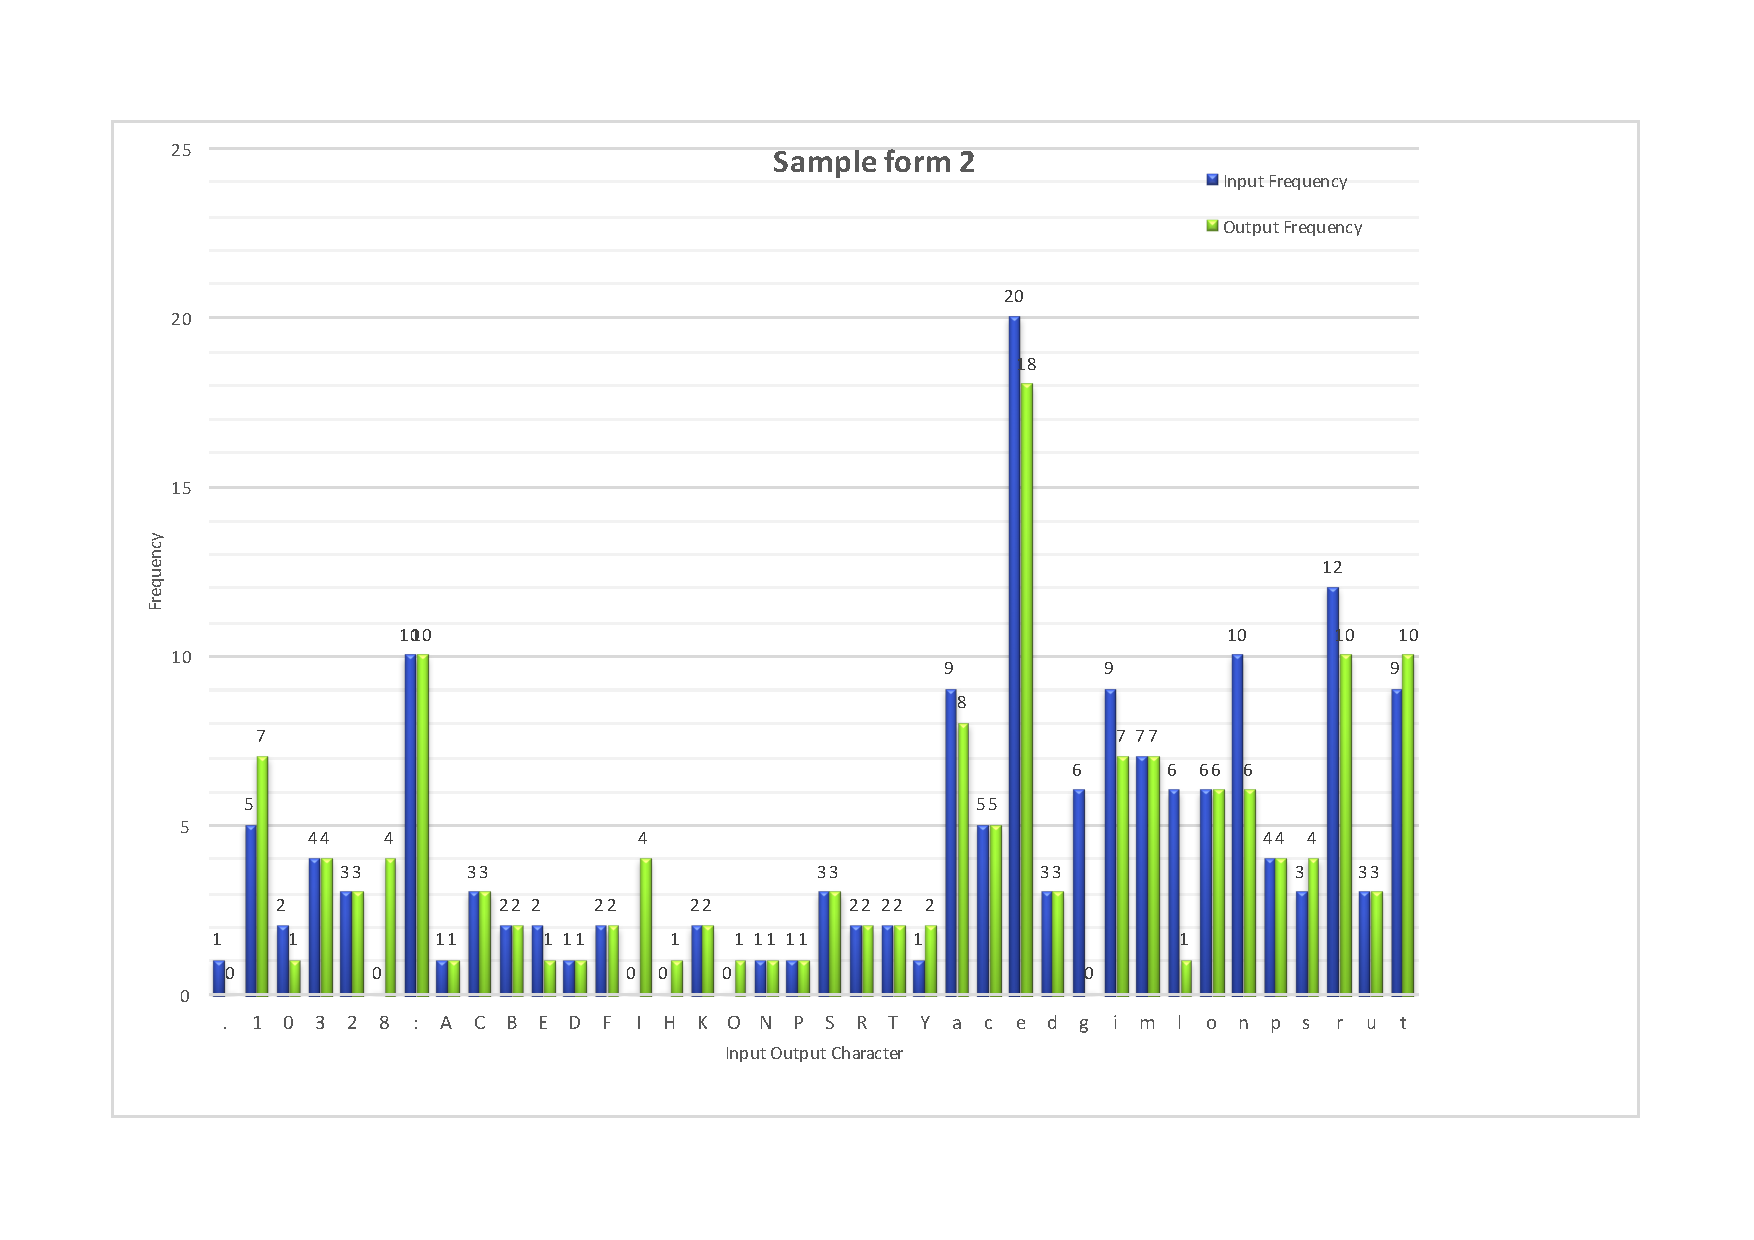
\includegraphics[width=1\textwidth]{form2.pdf}
\caption {Bar chart Input Output Frequency of Sample form 2}
\label {fig:bar2}
\end{figure}

\subsection{Sample form 3}

\begin{figure}[H]
\centering
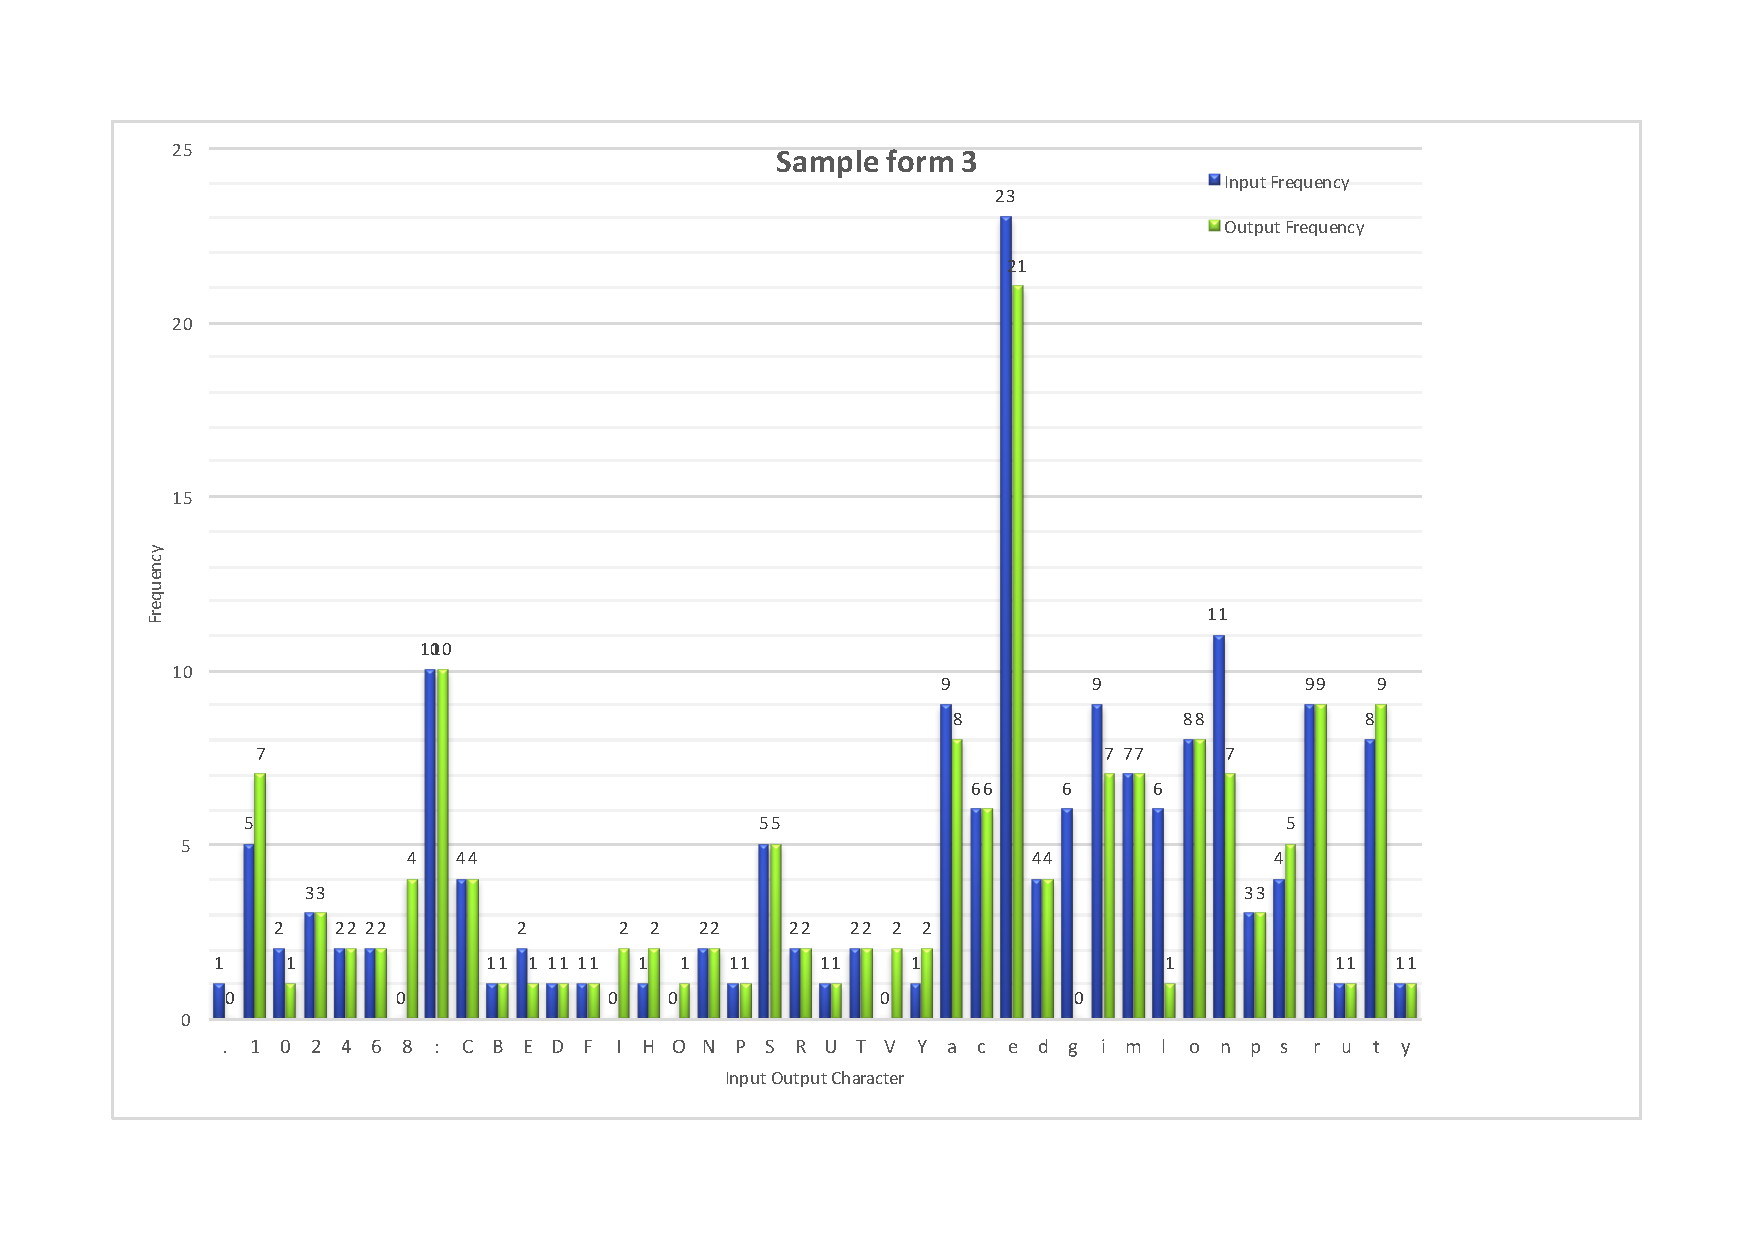
\includegraphics[width=1\textwidth]{form3}
\caption {Sample English form 3}
\label {fig:form3}
\end{figure}

\begin{table}[H]
\centering
\begin{tabular}{|p{2cm}|p{2cm}|p{2cm}|}
\hline
character & Input Frequency & Output Frequency \\
\hline
0 & 2 & 1\\
\hline
1 & 5 & 7\\
\hline
2 & 3 & 3\\
\hline
4 & 2 & 2\\ 
\hline
6 & 2 & 2\\
\hline
8 & 0 & 4\\
\hline
: & 10 & 10\\
\hline
B & 1 & 1\\
\hline
C & 4 & 4\\
\hline
D & 1 & 1\\
\hline
E & 2 & 1\\
\hline
F & 1 & 1\\
\hline
H & 1 & 2\\
\hline
I & 0 & 2\\
\hline
N & 2 & 2\\
\hline
O & 0 & 1\\
\hline
P & 1 & 1\\
\hline
R & 2 & 2\\
\hline
S & 5 & 5\\
\hline
T & 2 & 2\\
\hline
U & 1 & 1\\
\hline
V & 0 & 2\\
\hline
Y & 1 & 2\\
\hline
a & 7 & 8\\
\hline
c & 6 & 6\\
\hline
d & 4 & 4\\
\hline
e & 21 & 21\\
\hline
i & 9 & 7\\
\hline
l & 4 & 1\\
\hline
m & 7 & 7\\
\hline
n & 7 & 7\\
\hline
o & 8 & 8\\
\hline
p & 3 & 3\\
\hline
r & 9 & 9\\
\hline
s & 5 & 5\\
\hline
t & 9 & 9\\
\hline
u & 1 & 1\\
\hline
y & 1 & 1\\
\hline
\end{tabular}
\caption {Comparison between Input and Output frequency of Sample Input 3}
\label {tab:Table3}
\end{table}

\begin{figure}[H]
\centering
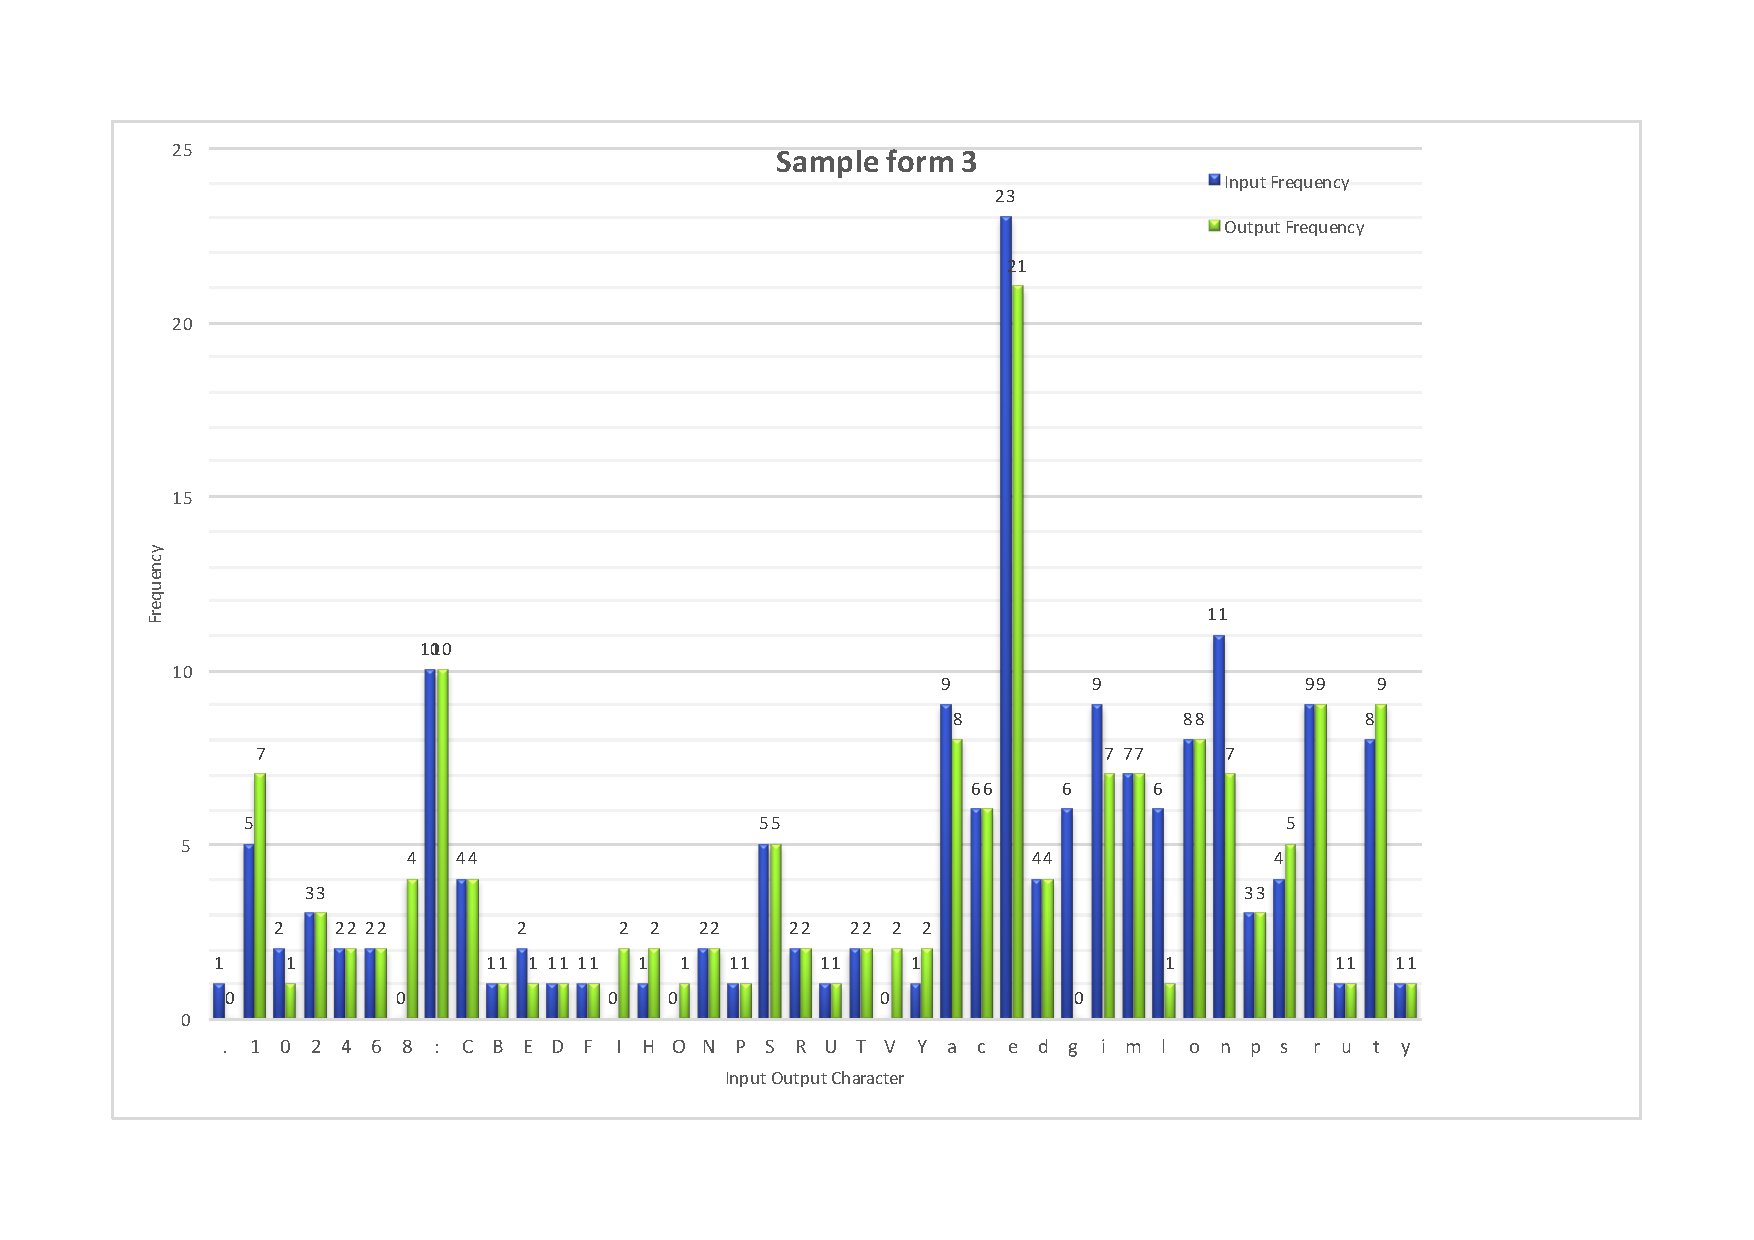
\includegraphics[width=1\textwidth]{form3.pdf}
\caption {Bar chart Input Output Frequency of Sample form 3}
\label {fig:bar3}
\end{figure}


\subsection{Sample form 4}

\begin{figure}[H]
\centering
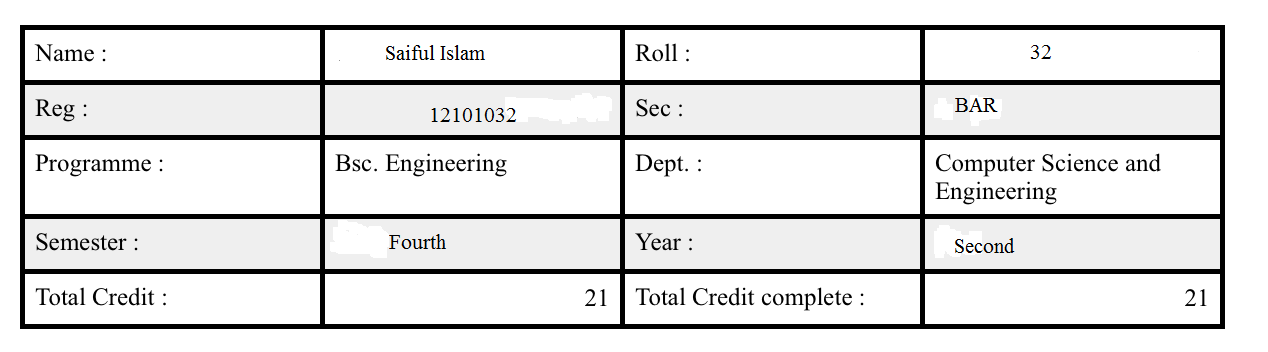
\includegraphics[width=1\textwidth]{form4}
\caption {Sample English form 4}
\label {fig:form4}
\end{figure}

\begin{table}[H]
\centering
\begin{tabular}{|p{2cm}|p{2cm}|p{2cm}|}
\hline
character & Input Frequency & Output Frequency \\
\hline
1 & 4  & 10\\
\hline
2 & 5  & 5\\
\hline
3 & 2  & 2\\
\hline
8 & 0  & 4\\
\hline
: & 10 & 10\\
\hline
A & 1  & 1\\
\hline
B & 1  & 2\\
\hline
C & 3  & 3\\
\hline
D & 1  & 1\\
\hline
E & 1  & 1\\
\hline
F & 1  & 1\\
\hline
H & 1  & 1\\
\hline
I & 2  & 2\\
\hline
N & 1  & 1\\
\hline
O & 2  & 2\\
\hline
P & 1  & 1\\
\hline
R & 3  & 3\\
\hline
S & 5  & 5\\
\hline
T & 2  & 2\\
\hline
Y & 2  & 2\\
\hline
a & 8  & 8\\
\hline
b & 1  & 1\\
\hline
c & c  & 6\\
\hline
d & 4  & 4\\
\hline
e & 17 & 19\\
\hline
f & 1  & 1\\
\hline
i & 6  & 6\\
\hline
l & 1  & 1\\
\hline
m & 7  & 7\\
\hline
n & 6  & 6\\
\hline
o & 2  & 8\\
\hline
p & 3  & 3\\
\hline
r & 8  & 8\\
\hline
s & 3  & 3\\
\hline
t & 9  & 10\\
\hline
u & 3  & 3\\
\hline
\end{tabular}
\caption {Comparison between Input and Output frequency of Sample Input 4}
\label {tab:Table4}
\end{table}

\begin{figure}[H]
\centering
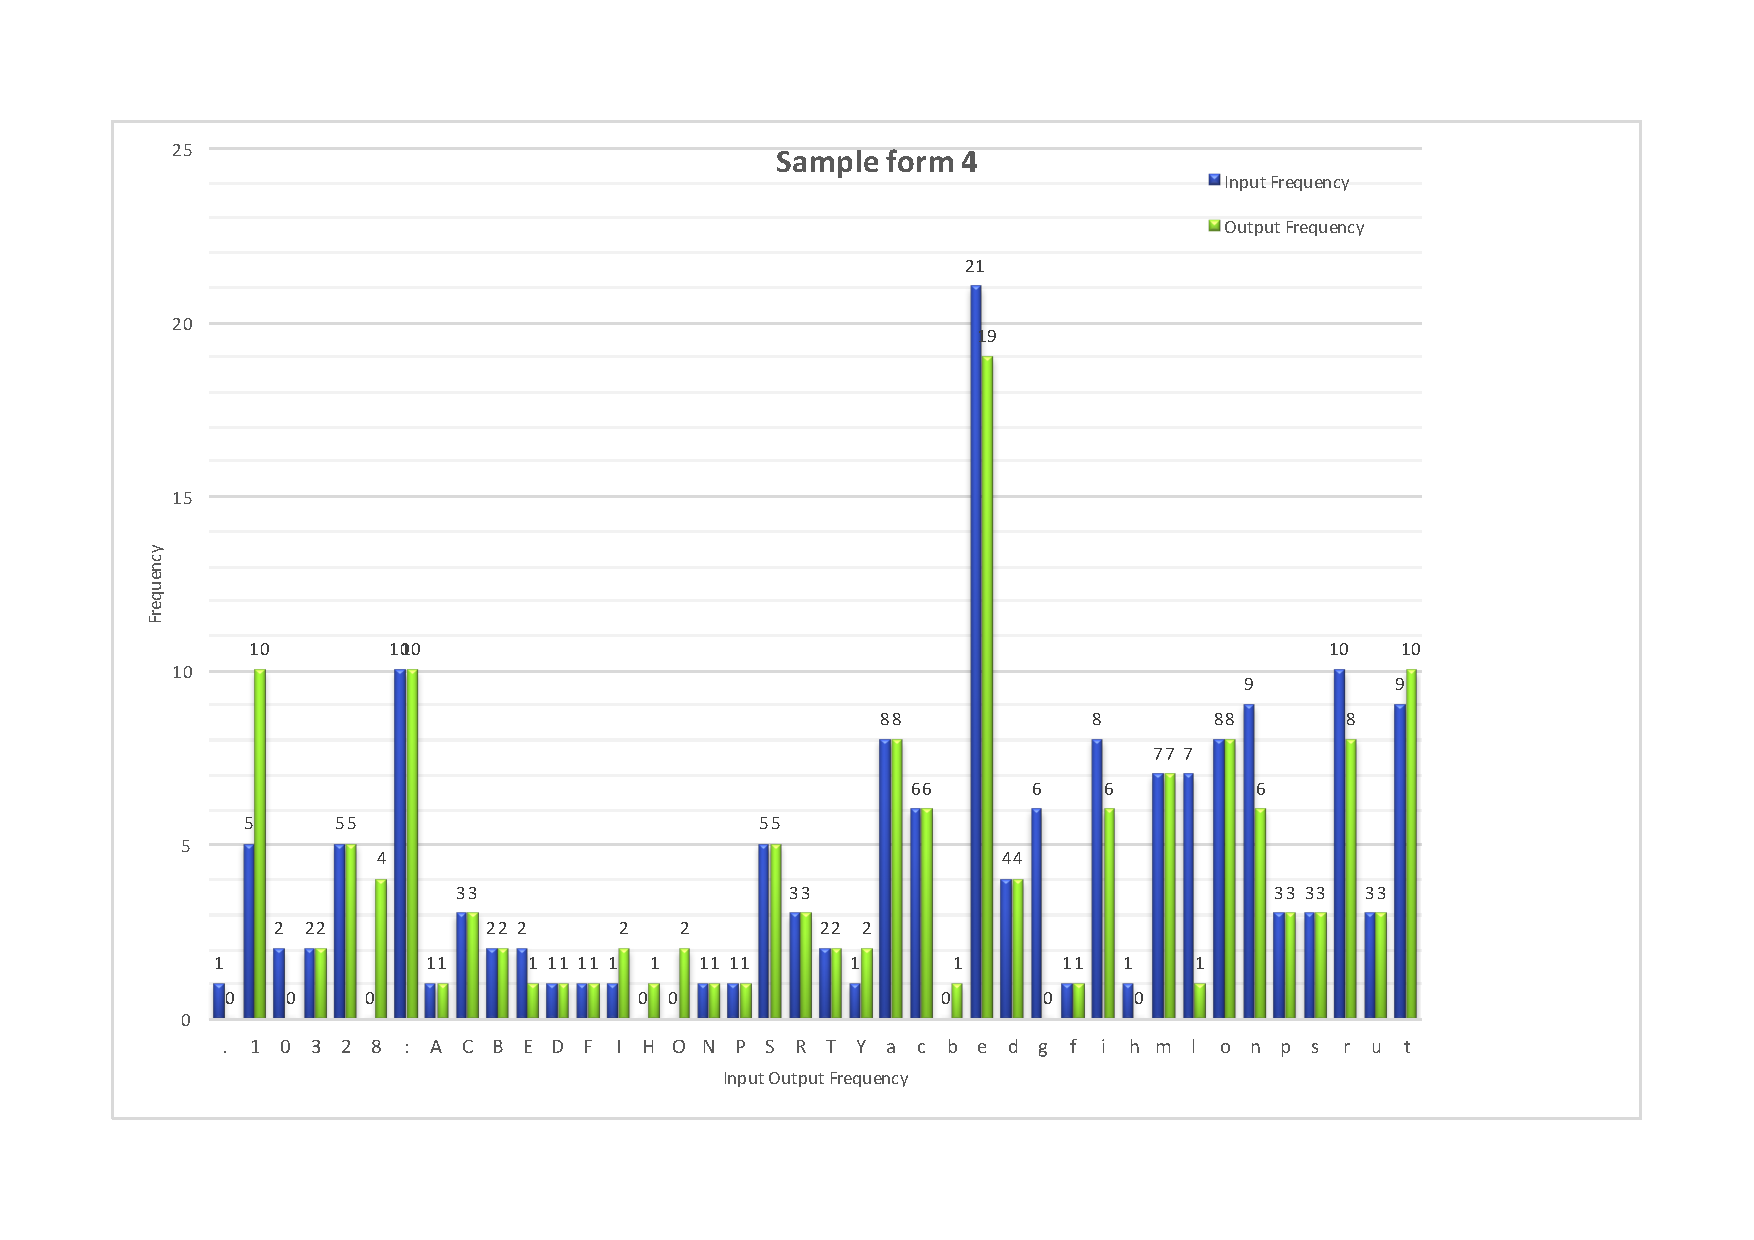
\includegraphics[width=1\textwidth]{form4.pdf}
\caption {Bar chart Input Output Frequency of Sample form 4}
\label {fig:bar4}
\end{figure}

\subsection{Sample form 5}

\begin{figure}[H]
\centering
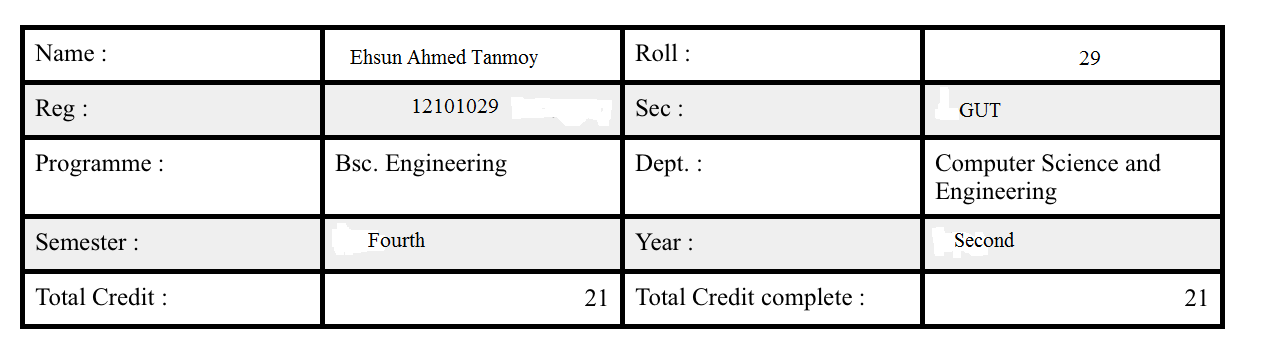
\includegraphics[width=1\textwidth]{form5}
\caption {Sample English form 5}
\label {fig:form4}
\end{figure}

\begin{table}[H]
\centering
\begin{tabular}{|p{2cm}|p{2cm}|p{2cm}|}
\hline
character & Input Frequency & Output Frequency \\
\hline
. & 1 & 0\\
\hline
1 & 5 & 7\\
\hline
0 & 2 & 0\\
\hline
2 & 5 & 5\\
\hline
9 & 2 & 2\\
\hline
8 & 0 & 4\\
\hline
: & 10 & 10\\
\hline
A & 1 & 1\\
\hline
C & 3 & 3\\
\hline
B & 1 & 1\\
\hline
E & 3 & 2\\
\hline
D & 1 & 1\\
\hline
G & 1 & 1\\
\hline
F & 1 & 1\\
\hline
I & 0 & 2\\
\hline
H & 0 & 1\\
\hline
L & 0 & 1\\
\hline
O & 0 & 2\\
\hline
N & 1 & 1\\
\hline
P & 1 & 1\\
\hline
S & 4 & 4\\
\hline
R & 2 & 2\\
\hline
U & 1 & 1\\
\hline
T & 4 & 4\\
\hline
Y & 1 & 2\\
\hline
a & 7 & 7\\
\hline
c & 6 & 6\\
\hline
b & 0 & 1\\
\hline
e & 22 & 20\\
\hline
d & 5 & 5\\
\hline
g & 6 & 0\\
\hline
i & 8 & 5\\
\hline
h & 2 & 2\\
\hline
m & 8 & 9\\
\hline
l & 5 & 1\\
\hline
o & 8 & 9\\
\hline
n & 11 & 8\\
\hline
p & 3 & 3\\
\hline
s & 4 & 3\\
\hline
r & 10 & 8\\
\hline
u & 2 & 2\\
\hline
t & 9 & 8\\
\hline
y & 1 & 1\\
\hline
\end{tabular}
\caption {Comparison between Input and Output frequency of Sample Input 5}
\label {tab:Table5}
\end{table}

\begin{figure}[H]
\centering
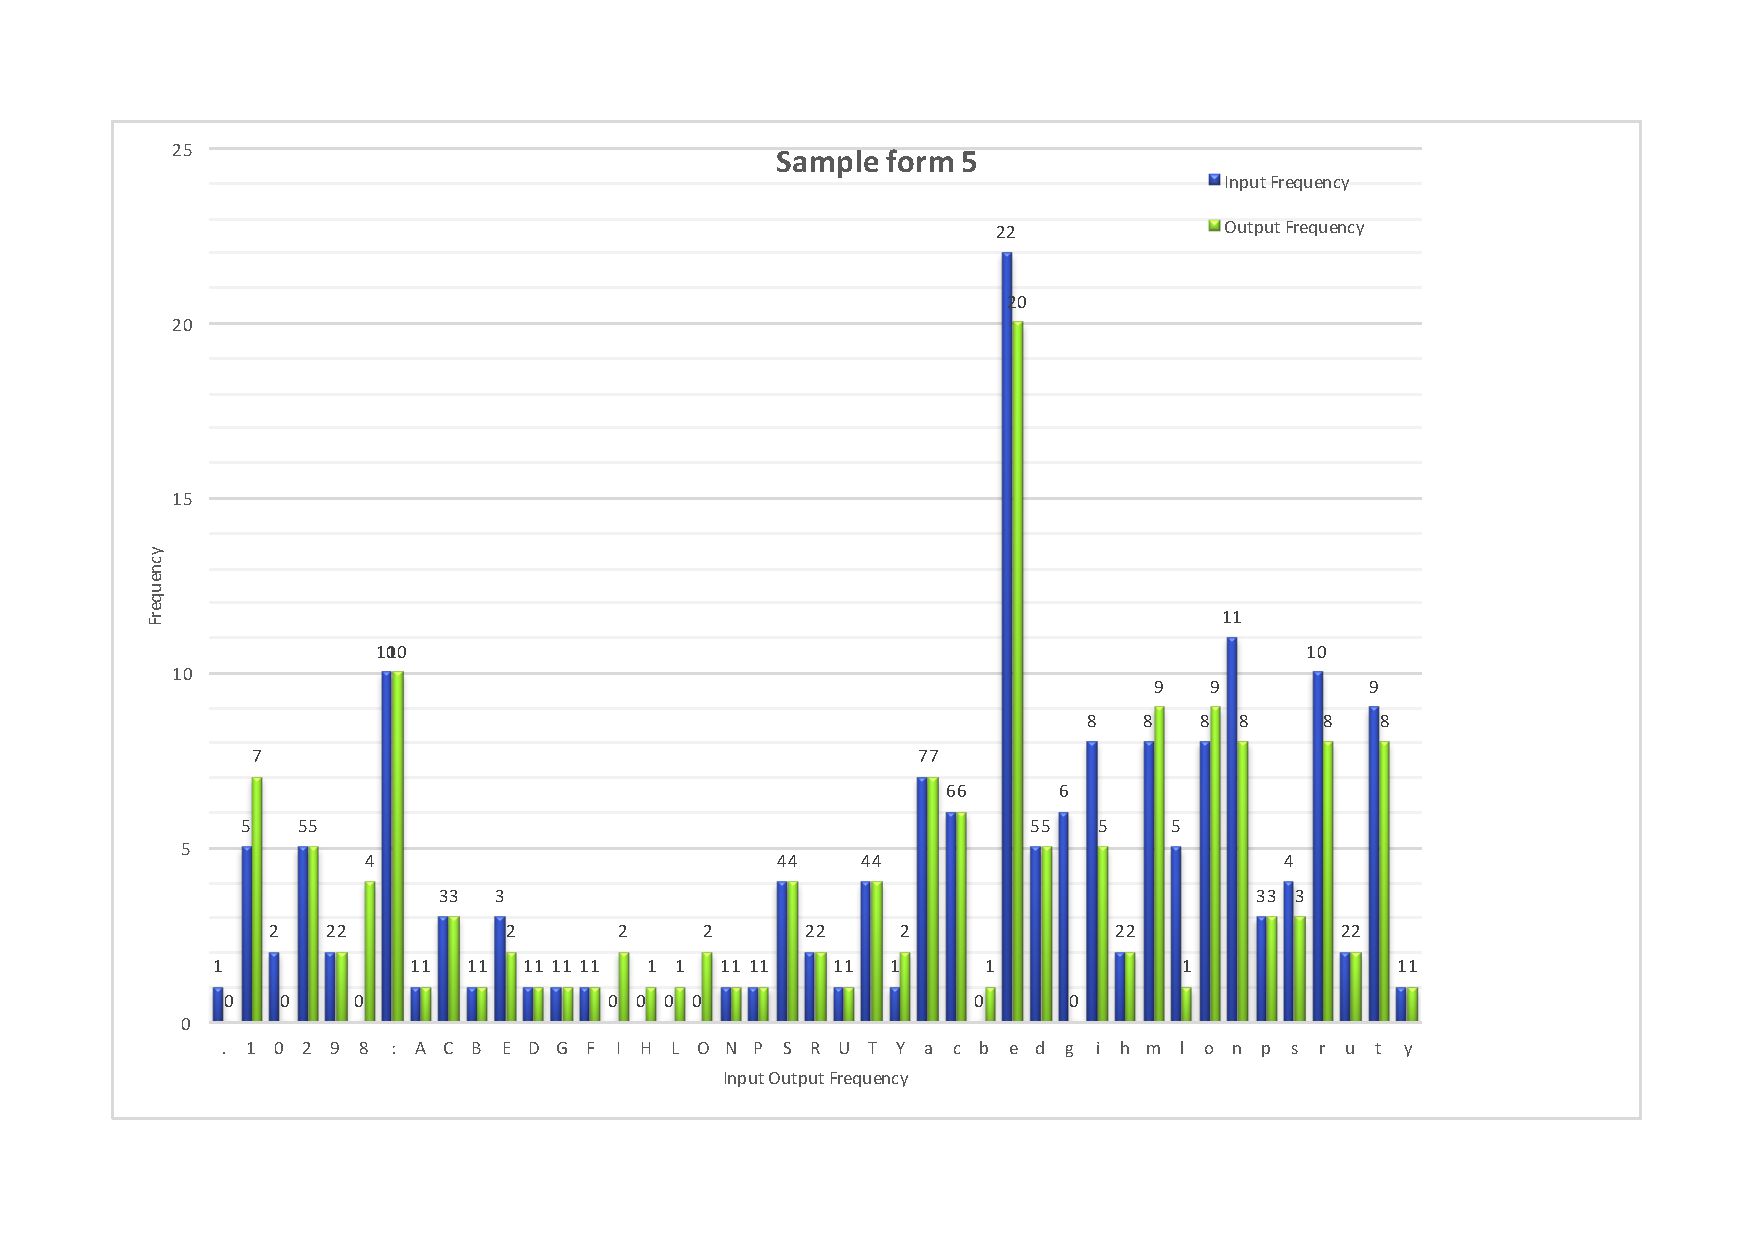
\includegraphics[width=1\textwidth]{form5.pdf}
\caption {Bar chart Input Output Frequency of Sample form 4}
\label {fig:bar5}
\end{figure}

According to these frequency table and bar chart we can say our tarined tesseract accuracy is upto 85\%. Here accuracy of character 'g' is below average. Most of the time character 'g' recognize as digit '8'. And double 'l' character (Ex: Roll) recognize as 'H'. It can be resolve with more frequent fonts training.

\section{Performance for Bangla form}
The result of Bangla form depends on the tesseract training data same as English form. For Bangla we train "Siyam rupali" font. Here we show our some output result and analysis of our training data.
\subsection{Sample form 1}
\begin{figure}[H]
\centering
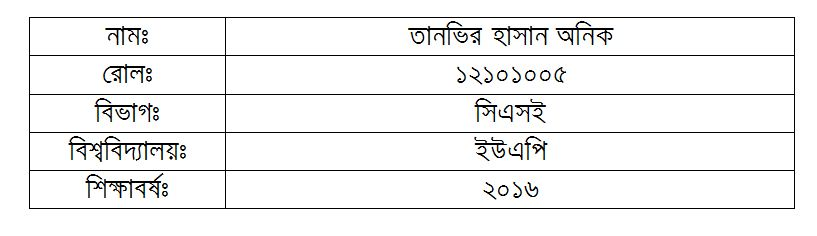
\includegraphics[width=1\textwidth]{formBen01.JPG}
\caption {Sample Bangla form 1}
\label {fig:FormBan1}
\end{figure}

\begin{table}[H]
\centering
\begin{tabular}{|p{2cm}|p{2cm}|p{2cm}|}
\hline
character & Input Frequency & Output Frequency \\
\hline
{\bengalifont ঃ} & 3 & 5\\
\hline
{\bengalifont অ} & 1 & 1\\
\hline
{\bengalifont ই} & 1 & 2\\
\hline
{\bengalifont উ} & 1 & 1\\
\hline
{\bengalifont এ} & 2 & 2\\
\hline
{\bengalifont ক} & 2 & 2\\
\hline
{\bengalifont গ} & 1 & 1\\
\hline
{\bengalifont চ} & 1 & 0\\
\hline
{\bengalifont ত} & 1 & 1\\
\hline
{\bengalifont '} & 8 & 0\\
\hline
{\bengalifont র} & 2 & 3\\
\hline
{\bengalifont ন} & 4 & 4\\
\hline
{\bengalifont প} & 1 & 1\\
\hline
{\bengalifont ভ} & 2 & 2\\
\hline
{\bengalifont ব} & 6 & 5\\
\hline
{\bengalifont য} & 2 & 1\\
\hline
{\bengalifont ম} & 1 & 1\\
\hline
{\bengalifont 0} & 4 & 0\\
\hline
{\bengalifont ল} & 4 & 2\\
\hline
{\bengalifont ষ} & 2 & 2\\
\hline
{\bengalifont শ} & 2 & 2\\
\hline
{\bengalifont হ} & 1 & 1\\
\hline
{\bengalifont স} & 1 & 3\\
\hline
{\bengalifont ;} & 1 & 0\\
\hline
{\bengalifont ়} & 1 & 0\\
\hline
{\bengalifont ি} & 8 & 7\\
\hline
{\bengalifont া} & 7 & 7\\
\hline
{\bengalifont ী} & 0 & 1\\
\hline
{\bengalifont ো} & 1 & 1\\
\hline
{\bengalifont ্} & 6 & 4\\
\hline
{\bengalifont য়} & 0 & 1\\
\hline
{\bengalifont ১} & 4 & 4\\
\hline
{\bengalifont ০} & 0 & 4\\
\hline
{\bengalifont ২} & 2 & 2\\
\hline
{\bengalifont ৫} & 1 & 1\\
\hline
{\bengalifont দ} & 1 & 1\\
\hline
{\bengalifont ৬} & 1 & 1\\
\hline
\end{tabular}
\caption { Comparison between Input and Output frequency of Sample Input 1}
\label {tab:BTable1}
\end{table}

\begin{figure}[H]
\centering
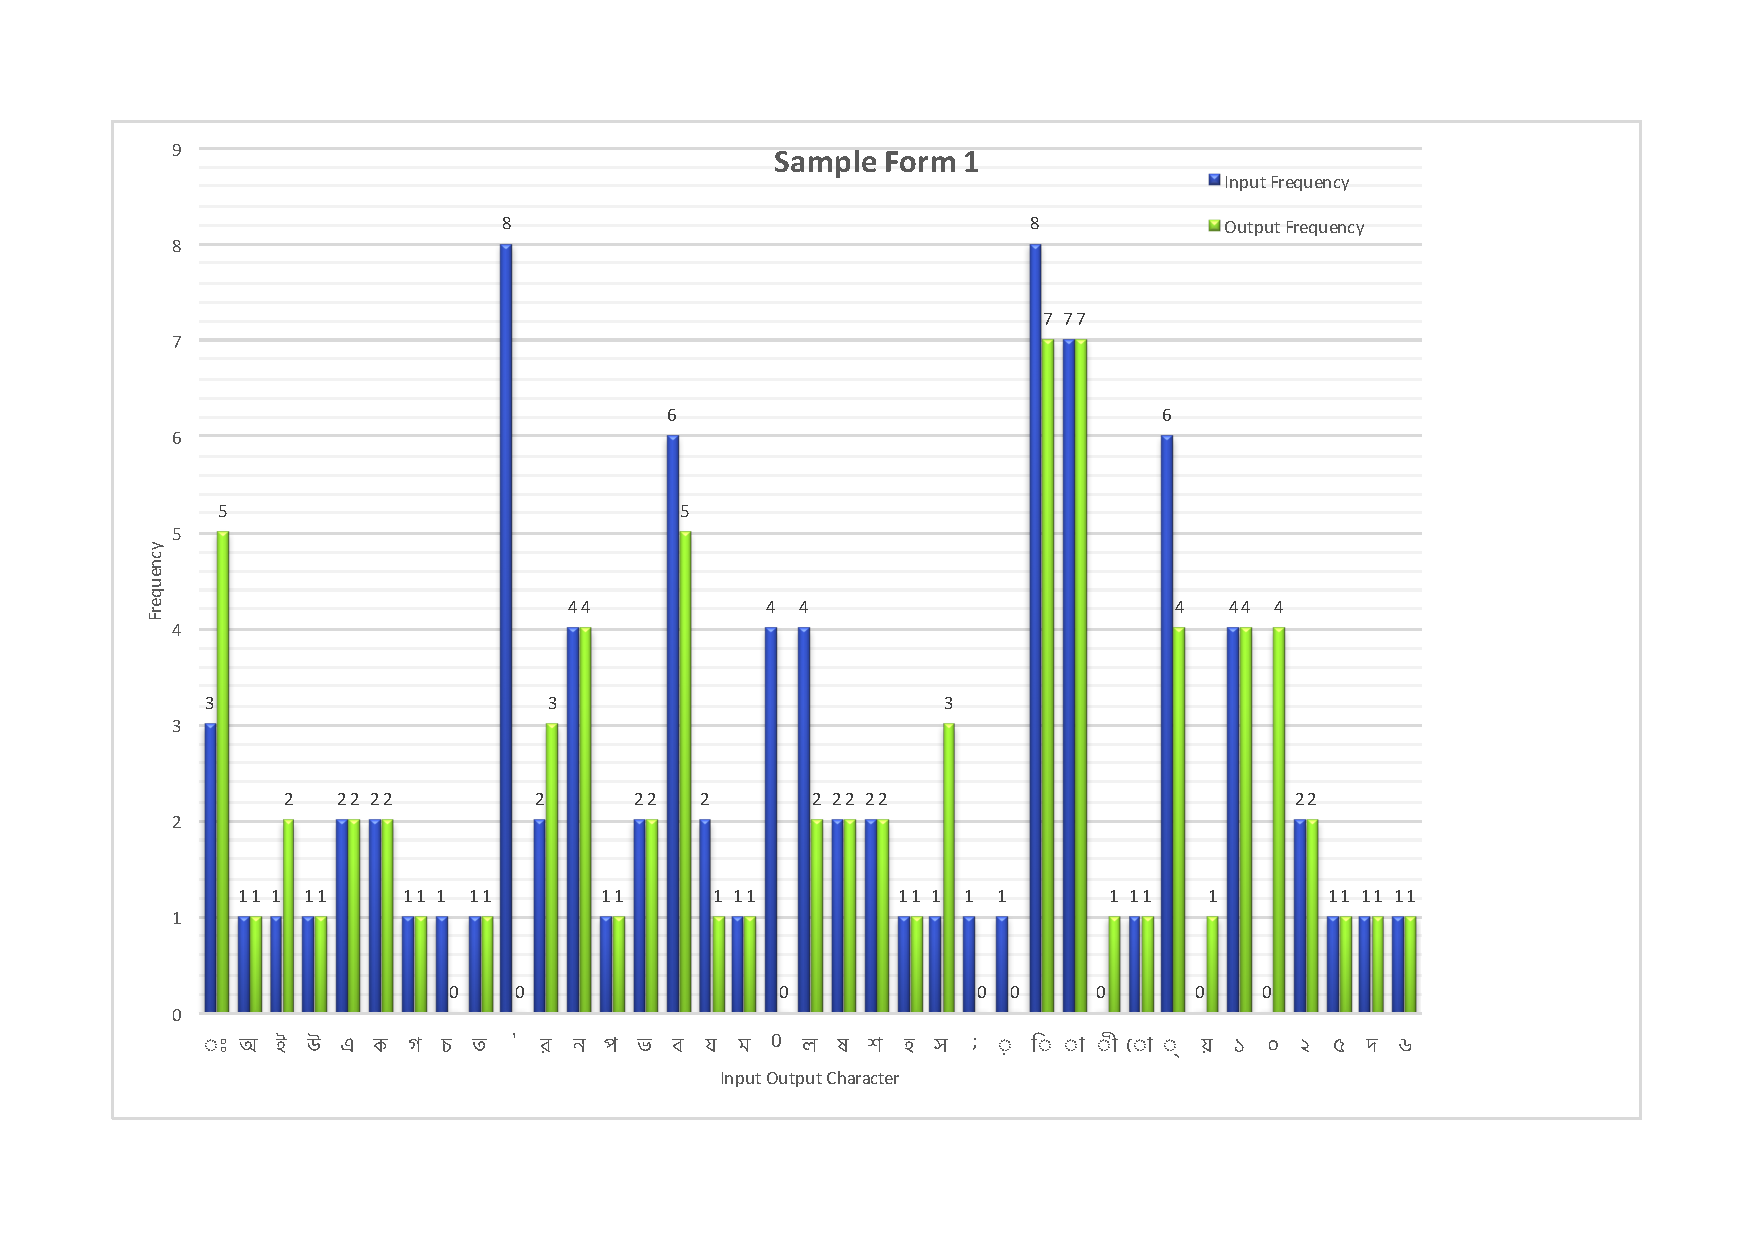
\includegraphics[width=1\textwidth]{Bform1.pdf}
\caption {Bar chart Input Output Frequency of Sample form 1}
\label {fig:Bbar1}
\end{figure}




\subsection{Sample form 2}
\begin{figure}[H]
\centering
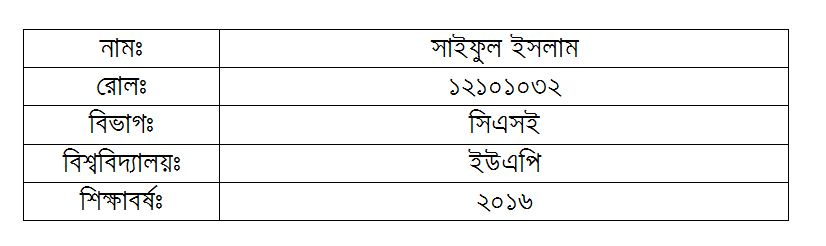
\includegraphics[width=1\textwidth]{formBen02.JPG}
\caption {Sample Bangla form 2}
\label {fig:FormBan2}
\end{figure}

\begin{table}[H]
\centering
\begin{tabular}{|p{2cm}|p{2cm}|p{2cm}|}
\hline
character & Input Frequency & Output Frequency \\
\hline
{\bengalifont ঃ} & 4 & 5\\
\hline
{\bengalifont ই} & 4 & 4\\
\hline
{\bengalifont উ} & 0 & 1\\
\hline
{\bengalifont ঊ} & 1 & 0\\
\hline
{\bengalifont এ} & 2 & 2\\
\hline
{\bengalifont ক} & 1 & 1\\
\hline
{\bengalifont গ} & 1 & 1\\
\hline
{\bengalifont ’} & 1 & 0\\
\hline
{\bengalifont চ} & 1 & 0\\
\hline
{\bengalifont '} & 7 & 0\\
\hline
{\bengalifont দ} & 1 & 1\\
\hline
{\bengalifont ন} & 1 & 1\\
\hline
{\bengalifont ফ} & 1 & 1\\
\hline
{\bengalifont প} & 1 & 1\\
\hline
{\bengalifont ভ} & 1 & 1\\
\hline
{\bengalifont ব} & 6 & 5\\
\hline
{\bengalifont য} & 2 & 1\\
\hline
{\bengalifont ম} & 2 & 2\\
\hline
{\bengalifont র} & 1 & 2\\
\hline
{\bengalifont ল} & 5 & 4\\
\hline
{\bengalifont ষ} & 2 & 2\\
\hline
{\bengalifont শ} & 2 & 2\\
\hline
{\bengalifont স} & 4 & 4\\
\hline
{\bengalifont ়} & 1 & 0\\
\hline
{\bengalifont ি} & 6 & 6\\
\hline
{\bengalifont া} & 6 & 6\\
\hline
{\bengalifont ু} & 1 & 1\\
\hline
{\bengalifont ে} & 1 & 0\\
\hline
{\bengalifont ো} & 1 & 1\\
\hline
{\bengalifont ্} & 6 & 4\\
\hline
{\bengalifont য়} & 0 & 1\\
\hline
{\bengalifont ১} & 4 & 4\\
\hline
{\bengalifont ০} & 3 & 3\\
\hline
{\bengalifont ৩} & 1 & 1\\
\hline
{\bengalifont ২} & 3 & 3\\
\hline
{\bengalifont ৬} & 1 & 1\\
\hline
\end{tabular}
\caption { Comparison between Input and Output frequency of Sample Input 2}
\label {tab:BTable2}
\end{table}


\begin{figure}[H]
\centering
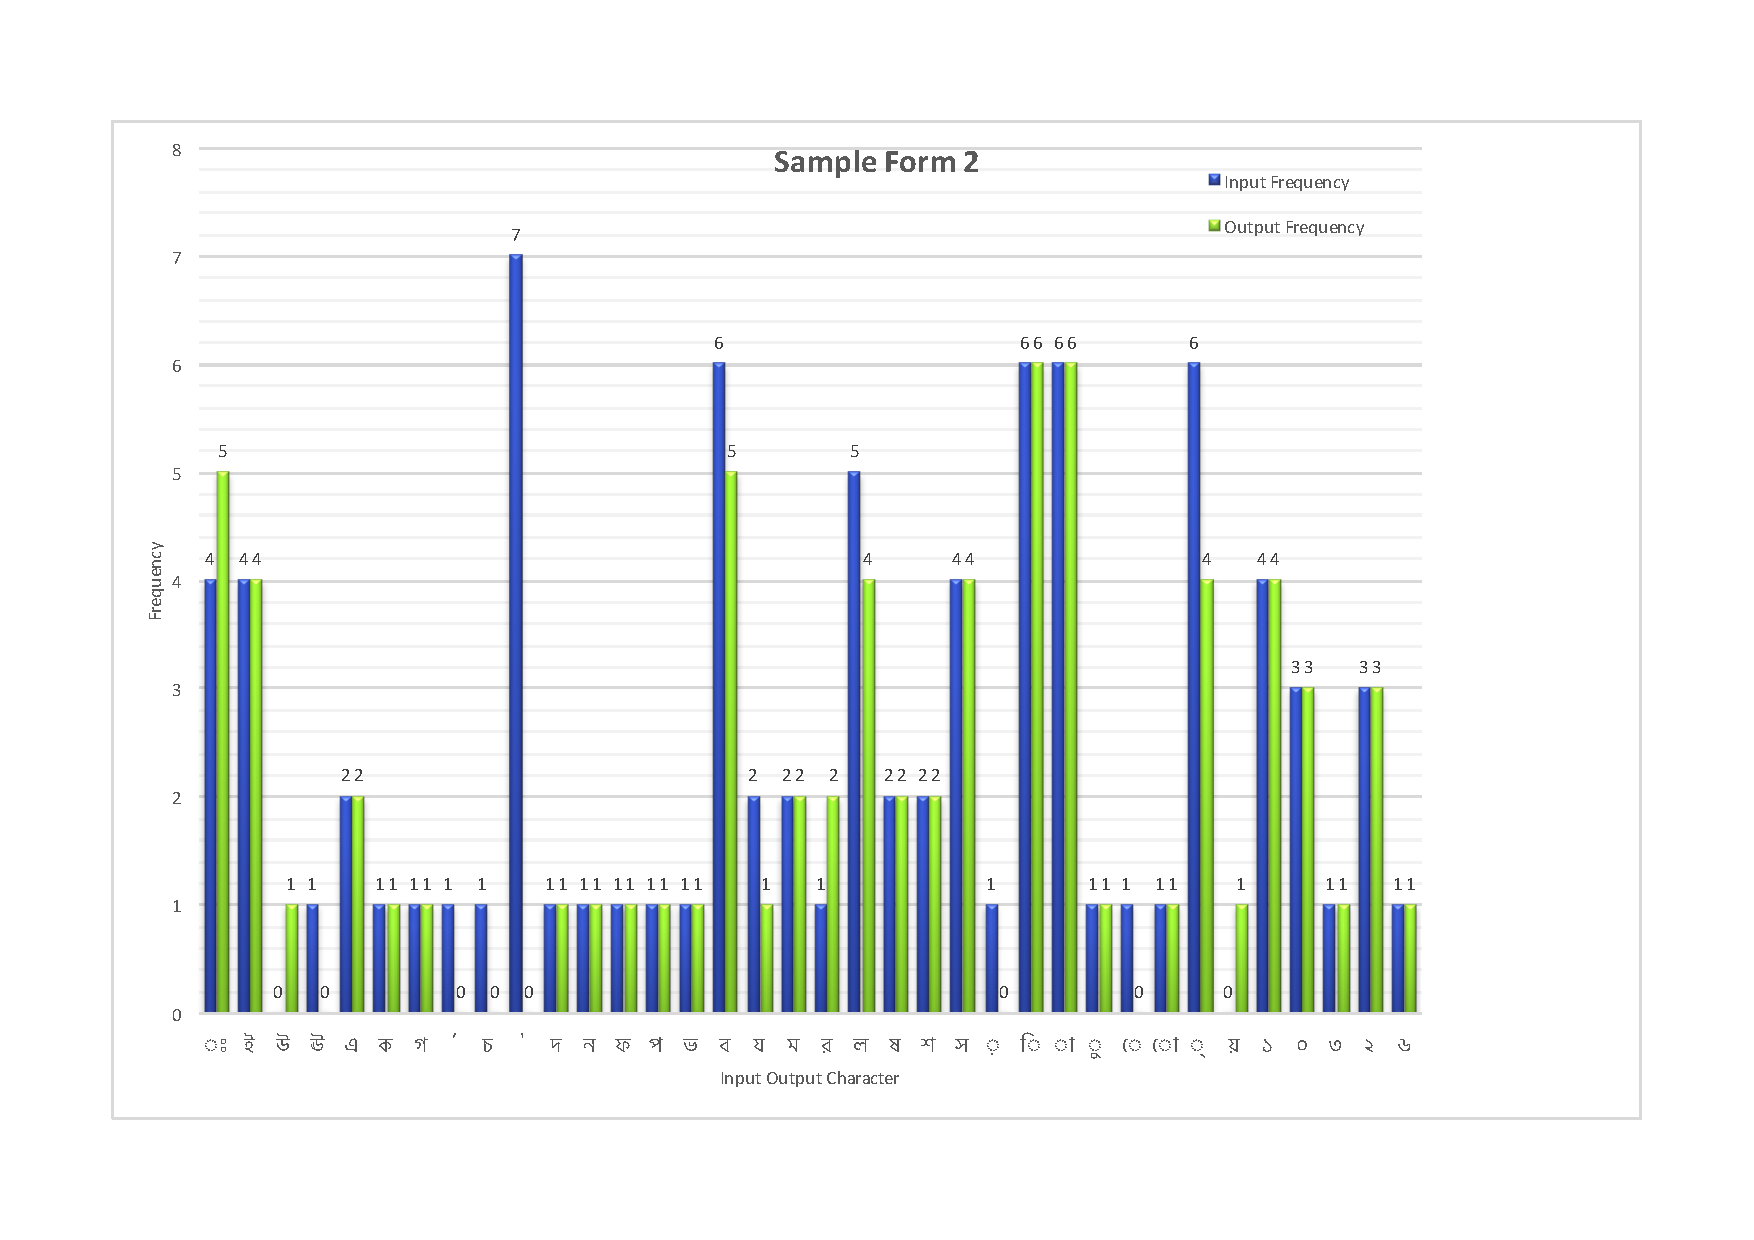
\includegraphics[width=1\textwidth]{Bform2.pdf}
\caption {Bar chart Input Output Frequency of Sample form 2}
\label {fig:Bbar2}
\end{figure}



\subsection{Sample form 3}
\begin{figure}[H]
\centering
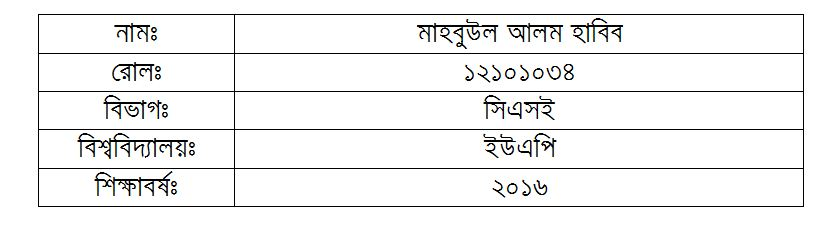
\includegraphics[width=1\textwidth]{formBen03.JPG}
\caption {Sample Bangla form 3}
\label {fig:FormBan3}
\end{figure}


\begin{table}[H]
\centering
\begin{tabular}{|p{2cm}|p{2cm}|p{2cm}|}
\hline
character & Input Frequency & Output Frequency \\
\hline
{\bengalifont ঃ} & 4 & 5\\
\hline
{\bengalifont ই} & 1 & 2\\
\hline
{\bengalifont আ} & 1 & 1\\
\hline
{\bengalifont উ} & 1 & 2\\
\hline
{\bengalifont ঊ} & 1 & 0\\
\hline
{\bengalifont এ} & 2 & 2\\
\hline
{\bengalifont ক} & 1 & 1\\
\hline
{\bengalifont গ} & 1 & 1\\
\hline
{\bengalifont ’} & 1 & 0\\
\hline
{\bengalifont চ} & 1 & 0\\
\hline
{\bengalifont '} & 8 & 0\\
\hline
{\bengalifont দ} & 1 & 1\\
\hline
{\bengalifont ন} & 1 & 1\\
\hline
{\bengalifont প} & 1 & 1\\
\hline
{\bengalifont ভ} & 1 & 1\\
\hline
{\bengalifont ব} & 9 & 8\\
\hline
{\bengalifont য} & 2 & 1\\
\hline
{\bengalifont ম} & 3 & 3\\
\hline
{\bengalifont 0} & 1 & 0\\
\hline
{\bengalifont ল} & 6 & 4\\
\hline
{\bengalifont ষ} & 2 & 2\\
\hline
{\bengalifont শ} & 2 & 2\\
\hline
{\bengalifont হ} & 2 & 2\\
\hline
{\bengalifont 8} & 1 & 0\\
\hline
{\bengalifont ়} & 1 & 0\\
\hline
{\bengalifont ি} & 7 & 7\\
\hline
{\bengalifont া} & 6 & 6\\
\hline
{\bengalifont ু} & 1 & 1\\
\hline
{\bengalifont ো} & 1 & 1\\
\hline
{\bengalifont ্} & 6 & 4\\
\hline
{\bengalifont র} & 1 & 2\\
\hline
{\bengalifont স} & 0 & 2\\
\hline
{\bengalifont য়} & 0 & 1\\
\hline
{\bengalifont ১} & 4 & 4\\
\hline
{\bengalifont ০} & 2 & 3\\
\hline
{\bengalifont ৩} & 1 & 1\\
\hline
{\bengalifont ২} & 2 & 2\\
\hline
{\bengalifont ৪} & 0 & 1\\
\hline
{\bengalifont ৬} & 1 & 1\\
\hline
\end{tabular}
\caption { Comparison between Input and Output frequency of Sample Input 3}
\label {tab:BTable3}
\end{table}

\begin{figure}[H]
\centering
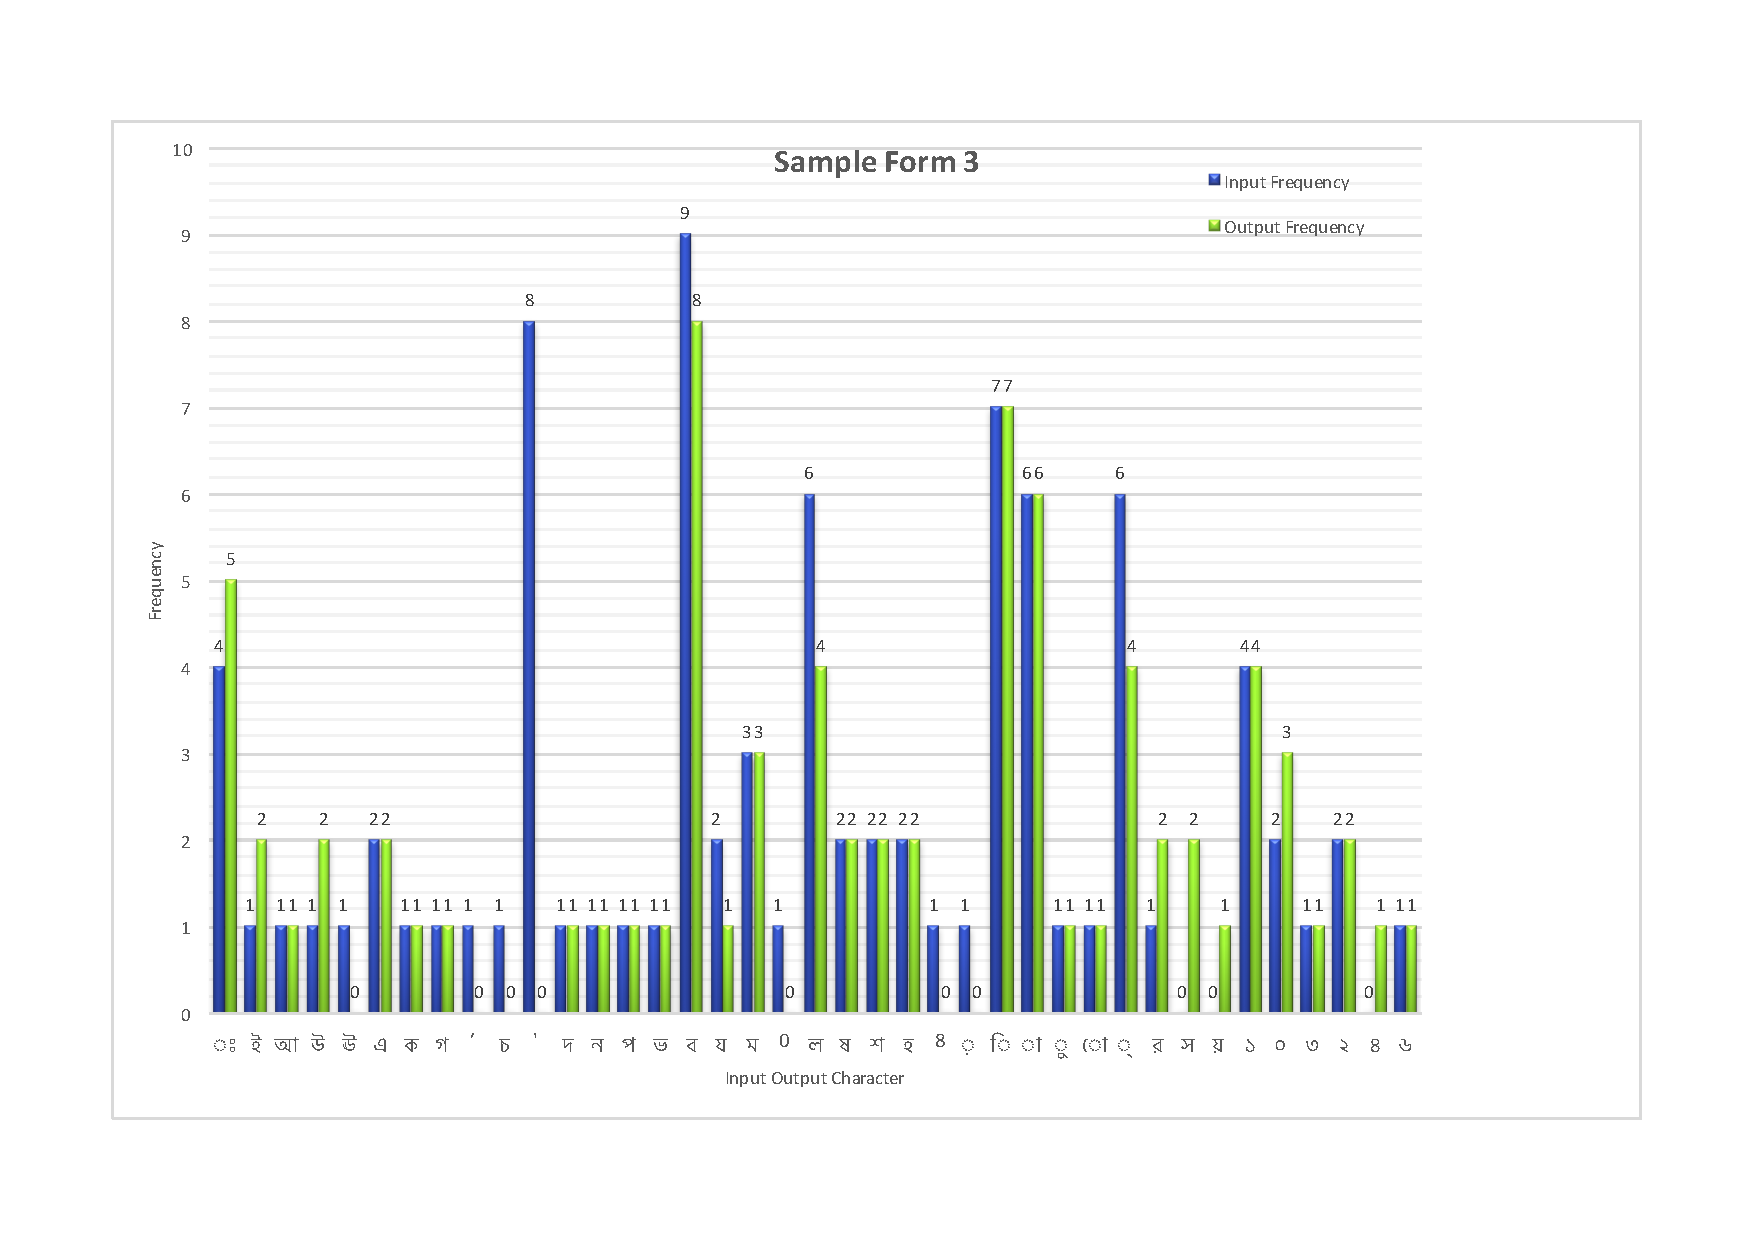
\includegraphics[width=1\textwidth]{Bform3.pdf}
\caption {Bar chart Input Output Frequency of Sample form 3}
\label {fig:Bbar3}
\end{figure}



\subsection{Sample form 4}
\begin{figure}[H]
\centering
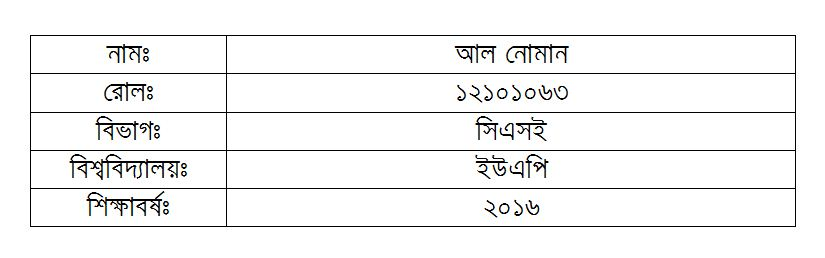
\includegraphics[width=1\textwidth]{formBen04.JPG}
\caption {Sample Bangla form 4}
\label {fig:FormBan4}
\end{figure}

\begin{table}[H]
\centering
\begin{tabular}{|p{2cm}|p{2cm}|p{2cm}|}
\hline
character & Input Frequency & Output Frequency \\
\hline
{\bengalifont ঃ} & 4 & 5\\
\hline
{\bengalifont ই} & 1 & 2\\
\hline
{\bengalifont আ} & 1 & 1\\
\hline
{\bengalifont উ} & 0 & 1\\
\hline
{\bengalifont ঊ} & 1 & 0\\
\hline
{\bengalifont এ} & 2 & 2\\
\hline
{\bengalifont ক} & 1 & 1\\
\hline
{\bengalifont গ} & 1 & 1\\
\hline
{\bengalifont ’} & 1 & 0\\
\hline
{\bengalifont চ} & 1 & 0\\
\hline
{\bengalifont '} & 8 & 0\\
\hline
{\bengalifont দ} & 1 & 1\\
\hline
{\bengalifont ন} & 3 & 3\\
\hline
{\bengalifont প} & 1 & 1\\
\hline
{\bengalifont ভ} & 1 & 1\\
\hline
{\bengalifont ব} & 6 & 5\\
\hline
{\bengalifont য} & 2 & 1\\
\hline
{\bengalifont ম} & 2 & 2\\
\hline
{\bengalifont র} & 1 & 2\\
\hline
{\bengalifont ল} & 5 & 3\\
\hline
{\bengalifont ষ} & 2 & 2\\
\hline
{\bengalifont শ} & 2 & 2\\
\hline
{\bengalifont স} & 0 & 2\\
\hline
{\bengalifont ়} & 1 & 0\\
\hline
{\bengalifont ি} & 6 & 6\\
\hline
{\bengalifont া} & 6 & 5\\
\hline
{\bengalifont ে} & 1 & 0\\
\hline
{\bengalifont ো} & 1 & 2\\
\hline
{\bengalifont ্} & 6 & 4\\
\hline
{\bengalifont য়} & 0 & 1\\
\hline
{\bengalifont ১} & 4 & 4\\
\hline
{\bengalifont ০} & 3 & 3\\
\hline
{\bengalifont ৩} & 1 & 1\\
\hline
{\bengalifont ২} & 2 & 2\\
\hline
{\bengalifont ৬} & 2 & 2\\
\hline
\end{tabular}
\caption { Comparison between Input and Output frequency of Sample Input 4}
\label {tab:BTable4}
\end{table}

\begin{figure}[H]
\centering
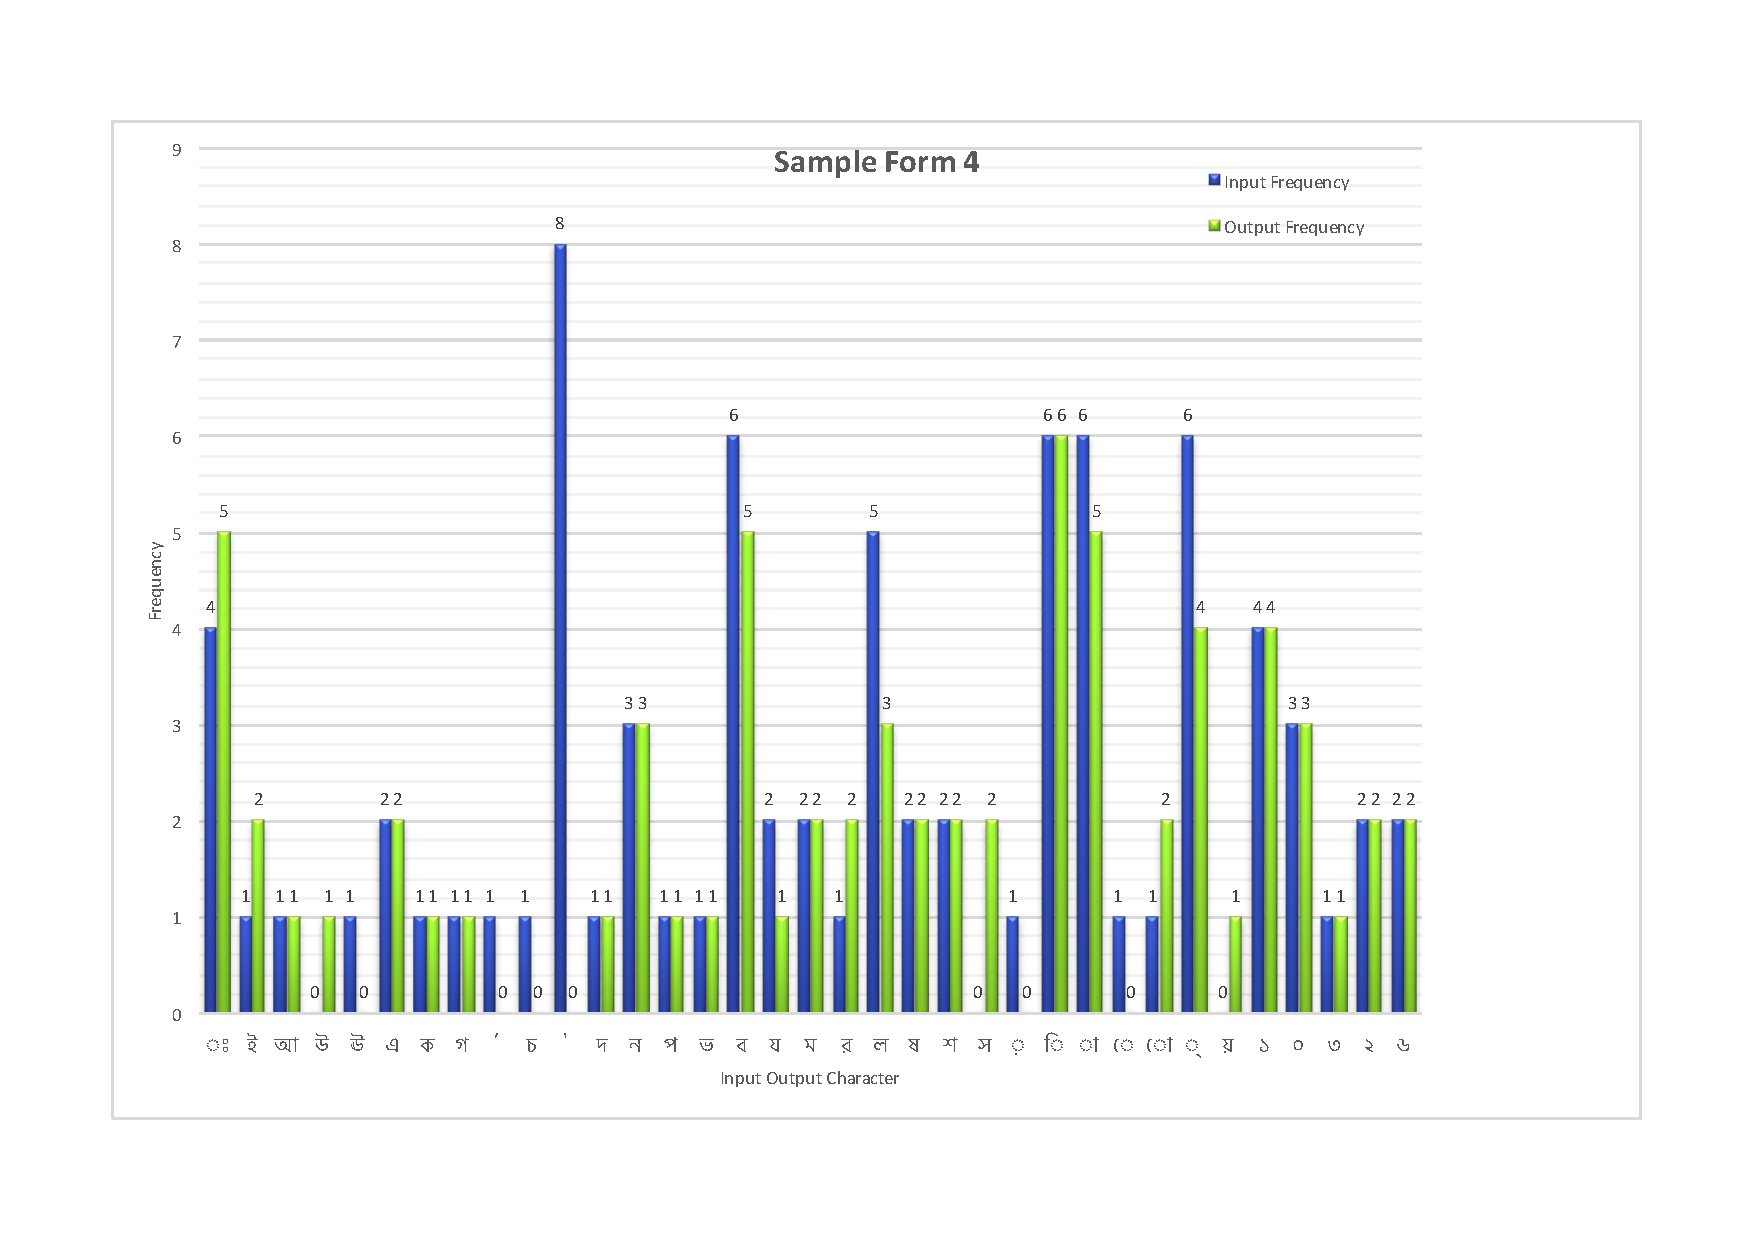
\includegraphics[width=1\textwidth]{Bform4.pdf}
\caption {Bar chart Input Output Frequency of Sample form 4}
\label {fig:Bbar4}
\end{figure}


\subsection{Sample form 5}
\begin{figure}[H]
\centering
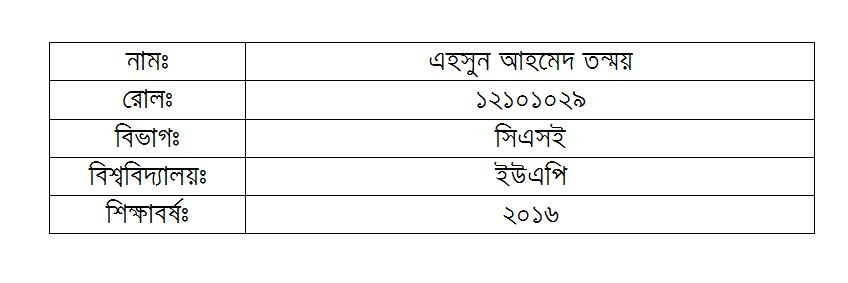
\includegraphics[width=1\textwidth]{formBen05.JPG}
\caption {Sample Bangla form 5}
\label {fig:FormBan5}
\end{figure}

\begin{table}[H]
\centering
\begin{tabular}{|p{2cm}|p{2cm}|p{2cm}|}
\hline
character & Input Frequency & Output Frequency \\
\hline
{\bengalifont ঃ} & 5 & 5\\
\hline
{\bengalifont 0} & 1 & 0\\
\hline
{\bengalifont ই} & 1 & 2\\
\hline
{\bengalifont আ} & 1 & 1\\
\hline
{\bengalifont উ} & 1 & 1\\
\hline
{\bengalifont এ} & 3 & 3\\
\hline
{\bengalifont ক} & 1 & 1\\
\hline
{\bengalifont গ} & 1 & 1\\
\hline
{\bengalifont ’} & 1 & 0\\
\hline
{\bengalifont চ} & 1 & 0\\
\hline
{\bengalifont ত} & 1 & 1\\
\hline
{\bengalifont '} & 7 & 0\\
\hline
{\bengalifont দ} & 2 & 2\\
\hline
{\bengalifont ন} & 4 & 3\\
\hline
{\bengalifont প} & 1 & 1\\
\hline
{\bengalifont ভ} & 1 & 1\\
\hline
{\bengalifont ব} & 6 & 5\\
\hline
{\bengalifont য} & 3 & 1\\
\hline
{\bengalifont ম} & 4 & 3\\
\hline
{\bengalifont র} & 1 & 2\\
\hline
{\bengalifont ল} & 4 & 2\\
\hline
{\bengalifont ষ} & 2 & 2\\
\hline
{\bengalifont শ} & 2 & 2\\
\hline
{\bengalifont হ} & 2 & 2\\
\hline
{\bengalifont স} & 1 & 3\\
\hline
{\bengalifont ়} & 2 & 0\\
\hline
{\bengalifont ি} & 6 & 6\\
\hline
{\bengalifont া} & 5 & 4\\
\hline
{\bengalifont ু} & 1 & 1\\
\hline
{\bengalifont ে} & 1 & 1\\
\hline
{\bengalifont ো} & 1 & 1\\
\hline
{\bengalifont ্} & 7 & 5\\
\hline
{\bengalifont য়} & 0 & 2\\
\hline
{\bengalifont ১} & 4 & 4\\
\hline
{\bengalifont ০} & 2 & 3\\
\hline
{\bengalifont ২} & 3 & 3\\
\hline
{\bengalifont ৬} & 1 & 1\\
\hline
{\bengalifont ৯} & 1 & 1\\
\hline
\end{tabular}
\caption { Comparison between Input and Output frequency of Sample Input 5}
\label {tab:BTable5}
\end{table}

\begin{figure}[H]
\centering
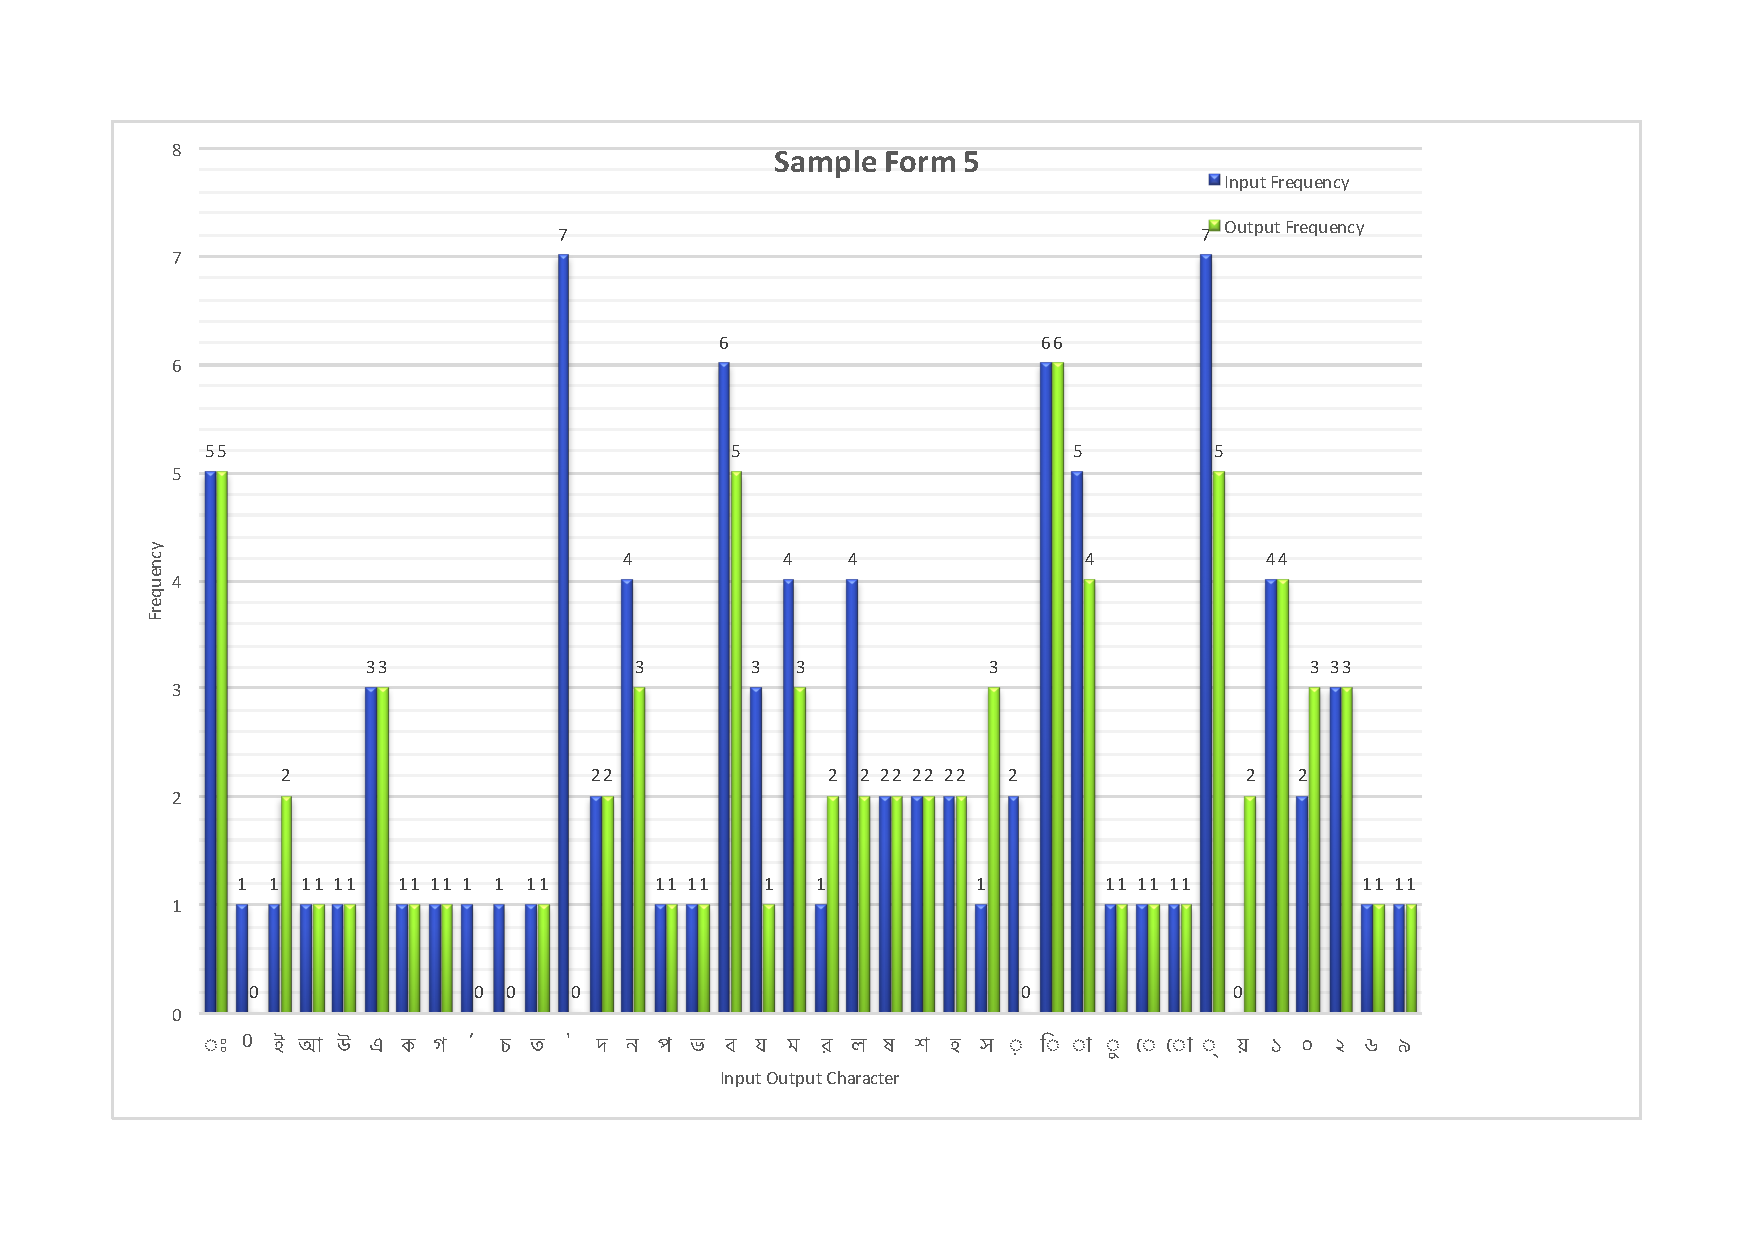
\includegraphics[width=1\textwidth]{Bform5.pdf}
\caption {Bar chart Input Output Frequency of Sample form 5}
\label {fig:Bbar5}
\end{figure}

According to these output of bangla from, we can say that here accuracy of our bangla tarining data upto 75\%. In our training data big problem is with complex bangla word. Our trained tesseract can't detect complex bangla word perfectly.


\chapter{Conclusion}
\label{chap:final}
This chapter summarizes the work presented in this thesis and figure out the advantages and limitations of the proposed algorithm. It also discussed about the scope of future works related to the proposed algorithm.
\section{Discussion}
From our experiments, we see that our methods could achieve the image segmentation purpose. For simple images with just a little texture inside, the result is quite good, and this method could also performs well on natural and landscape images. 
The above tests are based on the luminance or RGB based similarity measurement. When we test our algorithm on the texture images with the same similarity 
measurement, we found the result become worse. And the main reason is that the pixel value variance is really large in the texture region, which means pixels in the 
same texture region may have small similarities and are segmented into different groups.

This problem could be solved by using text on based similarity measurement,while the boundary position between segments are not so accurate determined due to the 
averaging operation by the sliding window.We knew that estimating the region properties is really an importance process. The Luminance-based method performs well on simple images with just a little texture inside.

And there’s bit of noise with the output. We’ve tried to reduce noise as much as possible but it's the particular area that we've still to work a lot.

Character recognition techniques associate a symbolic identity with the image of character. Character recognition is commonly referred to as optical character recognition (OCR), as it deals with the recognition of optically processed characters.

Optical character recognition has many different practical applications. As	observed from the experimental results,    Tesseract OCR engine fares reasonably with respect to the	core    recognition	accuracy	on    user-specific	handwritten   samples   of isolated/free-flow text. Developing high accuracy, multi-font language data for robust, end-to-end processing for Tesseract was not within the scope of this study.

\section{Future Works}

There are still some things we can do for future works. At first, we will improve the  stability of program. We want to modify the code of function to let programs more stable. Secondly, it’s a chance to get a better adaptive method for image segmentation even that we have an adaptive method already. The third one is to generate the post-processing mechanism for region merging. We can write a code about merging groups with the same texture into a single group.

As the computer technology develops new methods for character recognition are still expected to be appeared and hope that new methods will decrease the computational restrictions. For the recognition of joined and split characters integration of segmentation and contextual analysis can be improve. An important future work can be implemented, is to improve the training process to be able to use real data for training instead of just synthetic data with character bounding boxes. This will greatly help to improve the accuracy on Bengali handwritten forms.

Our work outputs multi-page TIFF format images and corresponding bounding box coordinates in the Tesseract training data format. So, to achieve more decent accuracy we need more training data. By adding more training data we’ll able to improve train data frequency, which we want do in near future.

Each and every aspects of our thesis can be improved upon. We just used our techniques to get a decent results but every techniques can be modified to get better result. For our thesis work, we just combining our techniques all together in order to achieve a decent result. There are many changes we would like to experiment with in the future.


%%
%% Make certain the ``references'' section begins on a recto page when
%% document is double-sided.
%% The ``bibliography'' line assumes that there is a file called
%% ``thesis.bib'' and that somewhere in the chapter material you have
%% cited something from it.
%%
\cleardoublepage
\bibliographystyle{unsrt}
\bibliography{thesis}
%%\include{appendices}

\end{document}
%% All Done!
